%%%% Preamble %%%%
\documentclass[a4paper, oneside]{article}

% wider text, smaller margins
\usepackage{a4wide}

\usepackage[utf8]{inputenc}
\usepackage[T1]{fontenc}
\usepackage{kpfonts}

% for coloring
\usepackage[dvipsnames]{xcolor}

% for index list
\usepackage{makeidx}
\makeindex

% for compact item lists
\usepackage{paralist}

% for hyperrefs
\usepackage{hyperref}

% for declaring math operators
\usepackage{amsthm}

% wrap text around figures
\usepackage{wrapfig}

% for compact lists
\usepackage{paralist}

% chagne format of section titles
\usepackage{titlesec}

% \titleformat*{\section}{\LARGE\bfseries}
% \titleformat*{\subsection}{\Large\bfseries}
% \titleformat*{\subsubsection}{\large\bfseries}
\titleformat*{\paragraph}{\bfseries\itshape}
% \titleformat*{\subparagraph}{\large\bfseries}

% nice text boxes
\usepackage{tcolorbox}
\newtcbox{\note}{on line, boxrule=0pt, boxsep=0pt, arc=0pt, outer arc=0pt, left=1pt, right=1pt, top=2pt, bottom=2pt, fontupper=\itshape}
\newtcolorbox{notebox}{boxrule=0pt}

% biblatex seetings for better referencing
\usepackage[backend=biber,
            citestyle=authoryear,
            bibstyle=numeric,
            block=space,
            backref=true,
            date=year,
            maxcitenames=2,
            mincitenames=1,
            url=false,
            doi=false,
            isbn=false,
            eprint=false]{biblatex}
\addbibresource{nf.bib}


%%% theorem environments
\theoremstyle{plain}
\newtheoremstyle{mytheoremstyle} % name
    {\topsep}{\topsep}{}{}%
    {\bfseries}% Theorem head font
    {}{.5em}%
    {\thmname{#1}\thmnumber{ #2}\thmnote{ (#3)}}  % Theorem head spec (can be left empty, meaning ‘normal’)
\theoremstyle{mytheoremstyle}
\newtheorem{theorem}{Theorem}[section]

\theoremstyle{definition}
\newtheoremstyle{mydefstyle} % name
    {\topsep}{\partopsep}{}{}%
    {\bfseries}% Theorem head font
    {}{.5em}%
    {\thmname{#1}\thmnumber{ #2}\thmnote{ (#3)}}  % Theorem head spec (can be left empty, meaning ‘normal’)
\theoremstyle{mydefstyle}
\newtheorem{definition}{Definition}[section]

%%% new shorthand commands
\newcommand{\nn}{\nonumber \\}%

\newcommand{\tldr}{\textbf{TLDR: }}
\newcommand{\concl}{\textbf{Concluding remarks: }}

% argmin/max opearator
\DeclareMathOperator*{\argmin}{arg\,min}%
\DeclareMathOperator*{\argmax}{arg\,max}%
\DeclareMathOperator*{\kl}{KL}%
\DeclareMathOperator*{\diag}{diag}%

% shortands for common math
\newcommand{\KL}[2]{\kl \left( #1 \parallel #2 \right)}
\newcommand{\pc}[2]{p \left( #1 \mid #2 \right)}
\newcommand{\abs}[1]{\lvert #1 \rvert}
\newcommand{\norm}[1]{\lVert #1 \rVert}
\newcommand{\dif}{\; \text{d} }

\newcommand{\mE}{\mathbb{E}}%%
\newcommand{\rE}{\mathrm{E}}%% % expectation
\newcommand{\rH}{\mathrm{H}}%% % entropy
\newcommand{\rI}{\mathrm{I}}%% % information
\newcommand{\mP}{\mathbb{P}}%% probability of random events
\newcommand{\mR}{\mathbb{R}}%% % real nums
\newcommand{\mS}{\mathbb{S}}%% % sphere
\newcommand{\mT}{\mathbb{T}}%% % tori
\newcommand{\mcR}{\mathcal{R}}%%
\newcommand{\mN}{\mathbb{N}}%% % natural nums
\newcommand{\mzZ}{\mathbb{Z}}%% % integers

\newcommand{\mD}{\mathcal{D}}%%
\newcommand{\mL}{\mathcal{L}}%%
\newcommand{\mM}{\mathcal{M}}%%
\newcommand{\mX}{\mathcal{X}}%%
\newcommand{\mY}{\mathcal{Y}}%%
\newcommand{\mZ}{\mathcal{Z}}%%

\newcommand{\ba}{\mathbf{a}}%%
\newcommand{\bb}{\mathbf{b}}%%
\newcommand{\bc}{\mathbf{c}}%%
\newcommand{\ff}{\mathbf{f}}%%
\newcommand{\bg}{\mathbf{g}}%%
\newcommand{\bh}{\mathbf{h}}%%
\newcommand{\bm}{\mathbf{m}}%%
\newcommand{\bp}{\mathbf{p}}%%
\newcommand{\bq}{\mathbf{q}}%%
\newcommand{\bs}{\mathbf{s}}%%
\newcommand{\bt}{\mathbf{t}}%%
\newcommand{\bu}{\mathbf{u}}%%
\newcommand{\bv}{\mathbf{v}}%%
\newcommand{\bw}{\mathbf{w}}%%
\newcommand{\bx}{\mathbf{x}}%%
\newcommand{\by}{\mathbf{y}}%%
\newcommand{\bz}{\mathbf{z}}%%
\newcommand{\pdx}{\mathbf{p_{\mD}(\bx)}}%%


\newcommand{\bB}{\mathbf{B}}%%
\newcommand{\bC}{\mathbf{C}}%%
\newcommand{\bH}{\mathbf{H}}%%
\newcommand{\bW}{\mathbf{W}}%%
\newcommand{\bX}{\mathbf{X}}%%
\newcommand{\bY}{\mathbf{Y}}%%
\newcommand{\bZ}{\mathbf{Z}}%%

% \newcommand{\note}[1]{\emph{\textbf{Note:} #1}}
% \newcommand{\idea}[1]{\emph{\textbf{\color{red}Idea:} #1}}


\begin{document}

% where pics are
\graphicspath{ {./Pics/} }

% supress paragraph idents
\setlength{\parindent}{0pt}
\setlength{\parskip}{1ex plus 0.5ex minus 0.2ex}

% Number equations within a section
\numberwithin{equation}{section}

{\large Magda's notes about \textbf{normalizing flows}}

{\hfill Last update: \today}

Informal notes for my future self who is likely to forget.
I explain the papers the way I understand them, using terminology and logic natural to me.
This means I may deviate from the original paper structure, notation, etc.
At places, my interpretation my be incorrect due to lack of understanding. 
I will strive for this not to happen too often but I'm certainly not infallible. 

This is a working document, not  polished, with possible typos, editing errors, etc. 


% Print table of contents
\tableofcontents

\clearpage

\section{Probability and measure theory}

This section contains the prerequisites of measure-theoric view of probability.
It is not a full recount of the theory, it only has bits and pieces as and when needed.

\begin{notebox}
Based mainly on \fullcite{siegristRandomProbabilityMathematical}

\hfill Notes taken: endJan - earlyFeb 2020 \index{February 2020}
\end{notebox}

%%%%%%%%%%%%%%%%%%%%%%%%%%%%%%%%%%%%%%%%%%%%%%%%%%%%%%
%%%%%%%%%%%%%%%%% Measure theory %%%%%%%%%%%%%%%%%%%%%
%%%%%%%%%%%%%%%%%%%%%%%%%%%%%%%%%%%%%%%%%%%%%%%%%%%%%%
\subsection{Measure theory}

\subsubsection{Measurable space}

\begin{definition}
A \textbf{$\sigma$-algebra}\index{$\sigma$-algebra} $\mathscr{S}$ of a set $S$ is a \emph{non-empty} collection of subsets of $S$ that is closed under a \emph{countable} number of set operations.
That is:
\begin{compactitem}
\item if $A \in \mathscr{S}$ then $A^c \in \mathscr{S}$
\item if $A_i \in \mathscr{S}$ for each $i$ in a countable index set $I$ then $\cup_{i \in I} A_i \in \mathscr{S}$.
\end{compactitem}
\end{definition}

Additional properties of \textbf{$\sigma$-algebra} $\mathscr{S}$
\begin{compactitem}
\item $S \in \mathscr{S}$ \hspace{0.5cm}
(Proof: For any $A \in \mathscr{S}$, we have $A^c \in \mathscr{S}$ and $S = A \cup A^c \in \mathscr{S}$.)
\item $\emptyset \in \mathscr{S}$ \hspace{0.5cm}
(Proof: From above $S \in \mathscr{S}$ and $S^c = \emptyset \in \mathscr{S}$.)
\item if $A_i \in \mathscr{S}$ for each $i$ in a countable index set $I$ then $\cap_{i \in I} A_i \in \mathscr{S}$ \hspace{0.5cm}
(Proof: If $A_i \in \mathscr{S}$ then $A_i^c \in \mathscr{S}$ and since $B = \cup_{i \in I} A_i^c \in \mathscr{S}$ then $B^c = \cap_{i \in I} A_i \in \mathscr{S}$.)
\end{compactitem}

\begin{definition}
A \textbf{measurable space}\index{measurable space} is the space $(S, \mathscr{S})$ consisting of a set $S$,  and the $\sigma$-algebra $\mathscr{S}$.
\end{definition}

\begin{definition}
A \textbf{Borel $\sigma$-algebra}\index{Borel $\sigma$-algebra} is the algebra $\sigma(\mathscr{S})$ generated by the open sets of the topological space $(S, \mathscr{S})$.

Note: Since closed sets are complements of open sets, the Borel $\sigma$-algebra contains the closed sets as well (and is in fact generated by the closed sets).
\end{definition}

\subsubsection{Measurable function}

\begin{definition}
Suppose sets $S$ and $T$ and a function $f : S \to T$.
If $A \subseteq T$, the \textbf{inverse image (pre-image)}\index{inverse image}\index{pre-image} of A under f is the subset of $S$ given by $f^{-1}(A) = \{x \in S : f(x) \in A\}$.

Note: Careful, though the notation is the same, the inverse image does not have to be a function (the inverse function may not exist).
\end{definition}

\begin{definition}
Suppose sets $S$ and $T$ and a function $f : S \to T$.
If $A \subseteq S$, the \textbf{forward (direct) image}\index{forward image}\index{direct image} of A under f is the subset of $T$ given by $f(A) = \{f(x) \in T : x \in A\}$.
\end{definition}

\begin{definition}
A \textbf{measurable function}\index{measurable function} is a function $f: S \to T$ where $(S, \mathscr{S})$ and $(T, \mathscr{T})$ are measurable spaces and $f^{-1}(A) \in \mathscr{S}$ for any $A \in \mathscr{T}$.

Note: a continuous function $f: S \to T$ is measurable.
\end{definition}

\subsubsection{Measure}

\begin{definition}
A \textbf{positive measure}\index{positive measure} on $(S, \mathscr{S})$ is the function $\mu : \mathscr{S} \to [0, \infty]$ such that:
\begin{compactitem}
\item $\mu(\emptyset) = 0$
\item if $\{A_i : i \in I \}$ is a countable, pairwise disjoint collection of sets on $\mathscr{S}$ then $\mu(\cup_{i \in I} A_i) = \sum_{i \in I} \mu(A_i)$ ($\sim$ \emph{countable additivity}\index{countable additivity}). 
\end{compactitem}
The triple $(S, \mathscr{S}, \mu)$ is a \textbf{measure space}\index{measure space}.
\end{definition}

\begin{theorem}[Push-forward measure]\index{push-forward measure}
Assume a measure space $(S, \mathscr{S}, \mu)$ a measurable space $(T, \mathscr{T})$ and a measurable function $f : S \to T$.
Then $\nu$ defined as below is a positive measure on $(T, \mathscr{T})$
\begin{equation*}
\nu(B) = \mu(f^{-1}(B)), \quad B \in \mathscr{T}
\end{equation*}
\end{theorem}

\begin{figure}[ht]
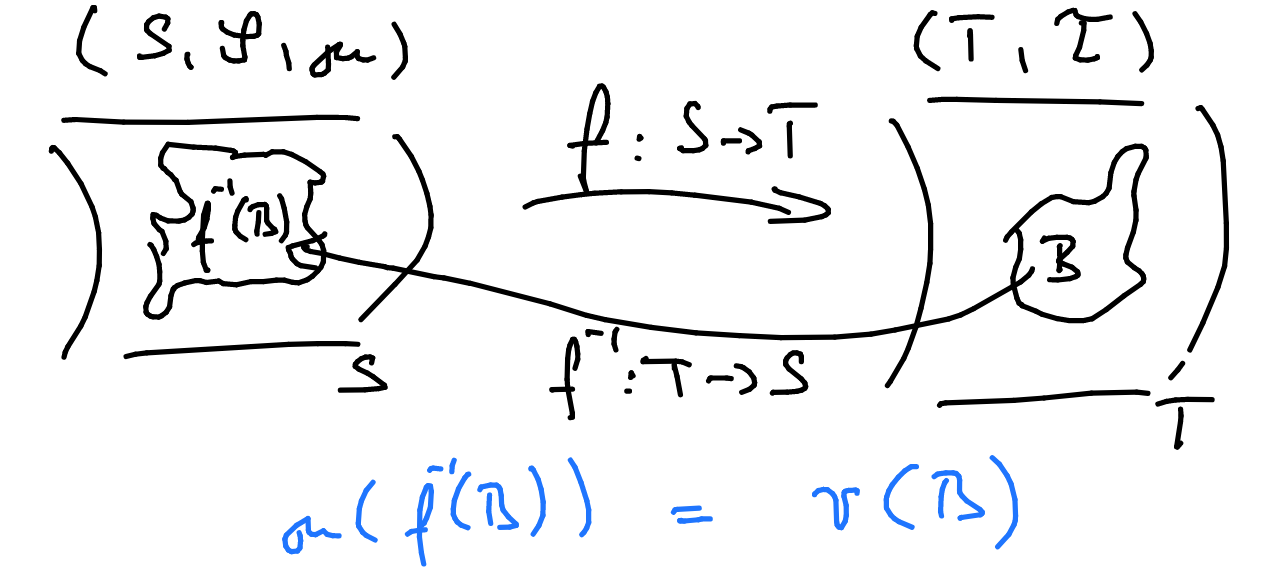
\includegraphics[width=0.5\textwidth]{changeOfVar}
\centering
\end{figure}

\begin{definition}
A \textbf{null set}\index{null set} of a measure space $(S, \mathscr{S}, \mu)$ is the set $A \in \mathscr{S}$ such that $\mu(A) = 0$.
\end{definition}

\begin{definition}
Consider a statement with $x \in S$ as a free variable.
\begin{compactitem}
\item The statement \textbf{holds on} $A$ if it is true for every $x \in A$
\item The statement \textbf{holds almost everywhere on} $A$\index{almost everywhere} (with respect to $\mu$) if there exists $B \in \mathscr{S}$ with $B \subseteq A$ such that the statement holds on B and $\mu(A \backslash B) = 0$ (\emph{null set}).
\end{compactitem}
\end{definition}


\begin{definition}
Sets $A, B \in \mathscr{S}$ are \textbf{equivalent}\index{equivalent sets} ($A \equiv B$) if $\mu(A \backslash B) + \mu(B \backslash A) = 0$ (the set of elements in which these two differ has measure zero).

Two measurable functions $f, g : S \to T$ are equivalent if $\mu\{x \in S : f(x) \neq g(x)\} = 0$ (the functions are only different over a set of x with measure zero).
\end{definition}

\begin{definition}
Suppose $\mu$ and $\nu$ are measures on $(S, \mathscr{S})$
\begin{compactenum}[a.]
\item $\nu$ is \textbf{absolutely continuous}\index{absolutely continuous measure} with respect to $\mu$ if every null set of $\mu$ is also a null set of $\nu$. We write $\nu \ll \mu$.
\item $\nu$ and $\mu$ are \textbf{mutually singular}\index{mutually singular measures} if there exists $A \in \mathscr{S}$ such that $A$ is null for $\mu$ and $A^c$ is null for $\nu$. We write $\mu \perp \nu$.
\item $\nu$ and $\mu$ are \textbf{equivalent}\index{equivalent measures} if $\mu \ll \nu$ and $\nu \ll \mu$. We write $\mu \equiv \nu$.
\end{compactenum}
\end{definition}

%%%%%%%%%%%%%%%%%%%%%%%%%%%%%%%%%%%%%%%%%%%%%%%%%%%%%%
%%%%%%%%%%%%%% Some standard measures %%%%%%%%%%%%%%%%
%%%%%%%%%%%%%%%%%%%%%%%%%%%%%%%%%%%%%%%%%%%%%%%%%%%%%%
\subsubsection{Some standard measures}

\paragraph{Borel measure}

\begin{definition}
A topological space $(S, \mathscr{T})$ with $\mathscr{S} = \sigma(\mathscr{T})$ a Borel $\sigma$-algebra has a positive measure $\mu$ on $(S, \mathscr{S})$ called the \textbf{Borel measure}\index{Borel measure}. The triplet $(S, \mathscr{S}, \mu)$ is a \textbf{Borel measure space}\index{Borel measure space}.
\end{definition}

\paragraph{Lebesgue measure}

\begin{definition}[Lebesgue measure]
For the standard \emph{Euclidean space} $(\mathbb{R}, \mathscr{R})$, $\mathscr{R}$ is the Borel $\sigma$-algebra generated by the standard Euclidean topology (collection of open or closed intervals $\mathscr{I}$ on $\mathbb{R}$).

For $a \leq b \in \mR$ all of the intervals $(a, b), (a, b], [a, b), [a, b]$ have the same \textbf{length} $b-a$.
Intervals $(a, \infty), [a, \infty), (-\infty, a), (-\infty, a]$ have all \textbf{length} $\infty$ and so does $\mR$ itself.

There exists a unique measure $\lambda$ on $\mathscr{R}$ such that $\lambda(I) = length(I)$ for all $I \in \mathscr{I}$.
This is the \textbf{Lebesgue measure}\index{Lebesgue measure} on $(\mathbb{R}, \mathscr{R})$.
\end{definition}

\begin{definition}[Lebesgue measure]
In the \emph{n-dimensional Euclidean space} $(\mathbb{R}^n, \mathscr{R}_n)$, the $\sigma$-algebra $\mathscr{R}_n$ is the n-fold power of $\mathscr{R}$, the Borel $\sigma$-algebra on $\mR$.
That is $\mathscr{R}_n = \mathscr{R} \otimes \mathscr{R} \otimes \ldots \otimes \mathscr{R}$.
It is also the sigma algebra generated by the products of intervals $\mathscr{R}_n = \sigma\{I_1 \times I_2 \times \ldots \times I_n : I_j \in \mathscr{I}, j \in \{1, 2, \dots, n\} \}$.

For $n \in \mN_+$ the n-fold power of $\lambda$ denoted $\lambda_n$ is the \textbf{Lebesgue measure} on $(\mathbb{R}^n, \mathscr{R}_n)$. In particular $\lambda(A_1 \times A_2 \times \ldots \times A_n) = \lambda(A_1) \lambda(A_2) \cdots \lambda(A_n); \ A_1, \ldots, A_n \in \mathscr{R}$ so that $\lambda_n$ is the \emph{n-dimensional volume} of $A \in \mathscr{R}_n$.
\end{definition}

Note: important properties of Lebesgue measure:
\begin{description}
\item[Translation invariance] If $A \subset \mR^n$ and $h \in \mR^n$ then $A + h \subseteq \mR^n$ and $\lambda_n(A) = \lambda_n(A + h)$
\item[Linear transformation] For linear map $T : \mR^n \to \mR^n$ and $A \subseteq \mR^n$ we denote by $TA = \{Tx \in \mR^n : x \in A\}$. Then $\lambda_n(TA) = \abs{\det T} \, \lambda_n(A)$ (by the usual interpretation of determinant as measuring the scaling of the linear transformation).
\item[Nonlinear differentiable transformation] For differentiable map $f : \mR^n \to \mR^n$ and $A \subseteq \mR^n$ we denote by $f(A) = \{f(x) \in \mR^n : x \in A\}$. Then $\lambda_n(f(A)) = \abs{\det J_f} \, \lambda_n(A)$ where $J_f = d f_i / d x_j$ is the Jacobian matrix. (This is probably not quite precise - Jacobian evaluated at which point as a local linear approximation?)
\end{description}


\paragraph{Lebesgue-Stieltjes measure}

\begin{definition}
A function $F : \mR \to \mR$  that satisfies
\begin{compactitem}
\item $F$ is increasing: if $x \leq y$ then $F(x) \leq F(y)$
\item $F$ is continuous from the right: $\lim_{t \downarrow x} F(t) = F(x)$ for all $x \in \mR$
\end{compactitem}
is a \textbf{distribution function}\index{distribution function} on $\mR$.
\end{definition}

\begin{definition}
If $F$ is a distribution function on $\mR$ then there exists a unique measure $\mu$ on $\mathscr{R}$ that satisfies $\mu(a, b] = F(b) - F(a), \ -\infty \leq a \leq b \leq \infty$. It is called the \textbf{Lebesgue-Stieltjes measure}\index{Lebesgue-Stieltjes measure}.
\end{definition}

\paragraph{Counting measure}

\begin{definition}
Assume a finite set $S$ with a power set (set of all subsets) $\mathscr{P}(S)$.
For $A \subseteq S$, the cardinality $\#(A)$ is the number of elements in $A$. The function $\#$ on $\mathscr{P}(S)$ is called the \textbf{counting measure}\index{counting measure}. (It is the usual measure on discrete spaces.)
\end{definition}

\paragraph{Probability measure}

\begin{definition}\label{defpre:probMeasure}
Suppose a measurable space $(S, \mathscr{S})$. 
A \textbf{probability measure}\index{probability measure} $\mP$ is a \emph{positive measure} on $(S, \mathscr{S})$ such that $\mP(S) = 1$.

%%%%%%%%%%%%%%%%%%%%%%%%%%%%%%%%%%%%%%%%%%%%%%%%%%%%%%
%%%%%%%%%%%%%%%%%%%%%% Probability %%%%%%%%%%%%%%%%%%%
%%%%%%%%%%%%%%%%%%%%%%%%%%%%%%%%%%%%%%%%%%%%%%%%%%%%%%
\subsection{Probability space}


\begin{definition}
A \textbf{probability space}\index{probability space} $(S, \mathscr{S}, \mathbb{P})$ consists of a set of outcomes of a random experiment $S$, the $\sigma-$algebra of events $\mathscr{S}$, and the probability measure $\mathbb{P}$ on the sample space $(S, \mathscr{S})$.

Note: $(\Omega, \mathscr{F}, \mP)$ is often used as special notation for probability spaces 
\end{definition}


Note: Any finite positive measure $\mu$ on the sample space $(S, \mathscr{S})$ can be re-scaled into a probability measure as $\mP(A) = \mu(A) / \mu(S), \ A \in \mathscr{S}$.

Note: Probability measure and \textbf{probability distribution}\index{probability distribution} are equivalent terms.
\end{definition}

\begin{definition}[random variable]
Suppose that $(S, \mathscr{S}, \mathbb{P})$ is a probability space and $(T, \mathscr{T})$ is another measurable space.
A \textbf{random variable}\index{random variable} $X$ with values in $T$ is a \emph{measurable} function from $S$ to $T$ ($X: S \to T$).
\begin{compactitem}
\item the probability measure of $X$ (the \emph{probability distribution} of $X$) is the mapping $P : T \to [0, 1]$ given by $P : B \to \mP(X \in B)$ (push-forward measure).
\item the collection of events $\{ X \in B : B \in \mathscr{T} \}$ is a sub $\sigma$-algebra of $\mathscr{S}$ and it is the $\sigma$-algebra generated by $X$ denoted by $\sigma(X)$
\end{compactitem}
Note: measurability of $X$ ensure that the inverse image of $B$ under $X$ (that is $\{X \in B\} = \{s \in S : X(s) \in B\}$) is in $\mathscr{S}$ (and hence is a valid event in $S$) for all $B \in \mathscr{T}$.
\end{definition}

\begin{figure}[ht]
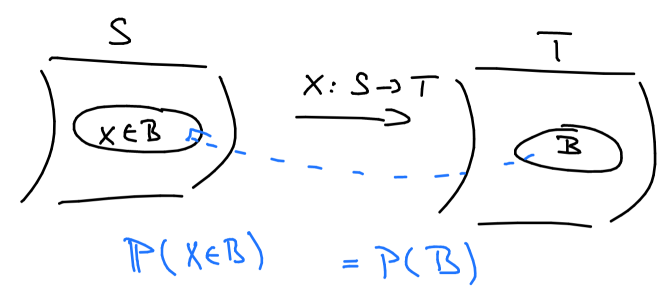
\includegraphics[width=0.5\textwidth]{probOfRV}
\centering
\end{figure}

\begin{definition}
Suppose that $(S, \mathscr{S}, \mathbb{P})$ is a probability space. 
Define the following collections of events
\begin{compactitem}
\item $\mathcal{N} = \{A \in \mathscr{S} : \mP(A) = 0\}$, the collection of \textbf{null} events\index{null events}
\item $\mathcal{M} = \{A \in \mathscr{S} : \mP(A) = 1\}$, the collection of \textbf{almost sure} events\index{almost sure events}
\item $\mathcal{D} = \mathcal{N} \bigcup \mathcal{M} = \{A \in \mathscr{S} : \mP(A) = 0 or \mP(A) = 1\}$, the collection of \textbf{essentially deterministic} events\index{essentially deterministic events}
\end{compactitem}
The collection of essentially deterministic events $\mathcal{D}$ is a sub $\sigma$-algebra of $\mathscr{S}$.
\end{definition}

\begin{definition}
Random variables $X$ and $Y$ taking values in in $T$ are \textbf{equivalent}\index{equivalent random variables} ($X \equiv Y$) if $\mP(X = Y) = 1$. Then
\begin{compactitem}
\item $\{X \in B\} \equiv \{Y \in B\}$ for every $B \in \mathscr{T}$
\item $X$ and $Y$ have the same probability distribution (measure) on $(T, \mathscr{T})$
\end{compactitem}
\end{definition}

\begin{definition}\label{defpre:probabilityDistributionFunc}
Suppose $X$ is a random variable with values in $\mR$. The \textbf{probability (cumulative) distribution function}\index{cumulative distribution function}\index{probability distribution function} of X is the function $F : \mR \to [0,1]$ defined by $F(x) = \mP(X \leq x), \ x \in \mR$.
\end{definition}

The probability distribution function has the following properties
\begin{compactitem}
\item F is increasing: if $x \leq y$ then $F(x) \leq F(y)$
\item F is continuous from the right: $F(x^+) = F(x)$
\item F has limits from the left: $F(x^-) = \mP(X < x)$
\item $F(-\infty) = 0$
\item $F(\infty) = 1$
\item If $X$ has continuous distribution on $\mR$ then $F$ is continuous.
\end{compactitem}

%%%%%%%%%%%%%%%%%%%%%%%%%%%%%%%%%%%%%%%%%%%%%%%%%%%%%%
%%%%%%%% Integral with respect to a measure %%%%%%%%%%
%%%%%%%%%%%%%%%%%%%%%%%%%%%%%%%%%%%%%%%%%%%%%%%%%%%%%%
\subsection{Integral with respect to a measure}

We denote the integral of a measurable function $f : S \to \mR$ with respect to a measure $\mu$ as either of the three (usually the first two)
\begin{equation}
\int_S f \dif \mu, \ \int_S f(x) \dif \mu(x), \int_S f(s) \, \mu(dx),
\end{equation}

\begin{definition}[Integral]
Suppose a measure space $(S, \mathscr{S}, \mu)$ with set $S$, $\sigma$-algebra $\mathscr{S}$ and positive measure $\mu$ on $\mathscr{S}$

\begin{enumerate}[a.]
\item For a simple function $f = \sum_{i \in I} a_i \mathbf{1}_{A_i}$ where $I$ is a finite index set and $a_i \in [0, \infty)$ and $A_i$ measurable partition of $S$ then
\begin{equation}
\int_S f \dif \mu = \sum_{i \in I} a_i \mu(A_i)
\end{equation}
Note: $\int_S \mathbf{1}_A \dif \mu = \mu(A)$ and $\int_S 0 \dif \mu = \int_S \mathbf{1}_{\emptyset} \dif \mu = 0$.

\item For a measurable $f : S \to [0, \infty)$
\begin{equation}
\int_S f \dif \mu = \sup \left\{ \int_S g \dif \mu : \text{ g is simple and } 0 \leq g \leq f \right\}
\end{equation}

\item For a measurable $f : S \to \mR$ with $f^+$ and $f^-$ denoting the positive and negative parts of $f$
\begin{equation}
\int_S f \dif \mu = \int_S f^+ \dif \mu - \int_S f^- \dif \mu
\end{equation}
as long as the right side does not form $\infty - \infty$.

\item For a measurable $f : S \to \mR$ and $A \in \mathscr{S}$, we define
\begin{equation}
\int_A f \dif \mu = \int_S \mathbf{1}_A f \dif \mu
\end{equation}
assuming that the right side exists.

\end{enumerate}
\end{definition}

\subsubsection{Integral with respect to some common measures}

\paragraph{Integration with respect to counting measure} $(S, \mathscr{S}, \#)$ is \emph{discrete} if $S$ is countable, $\mathscr{S}$ is collection of all subsets of $S$, and $\#$ is the counting measure on $\mathscr{S}$.
Then all $f : S \to \mR$ are measurable and integrals with respect to $\#$ are simply sums
\begin{equation}
\int_S f \dif \# = \sum_{x \in S} f(x) \enspace .
\end{equation}

\paragraph{Lebesgue integration} For the one-dimensional Euclidean space $(\mR, \mathscr{R}, \lambda)$ where $\mathscr{R}$ is the usual $\sigma$-algebra and $\lambda$ is the Lebesgue measure the \emph{Lebesgue} integral\index{Lebesgue integral} of a measurable function $f : \mR \to \mR$ over a set $A \in \mR$ is
\begin{equation}
\int_A f \dif \lambda
\end{equation}
Note: \textbf{Riemann}\index{Riemann integral} integral is denoted as $\int_a^b f(x) \dif x$. It can be shown that if function $f$ is Riemann integrable on an interval $[a, b]$ it is also Lebesgue integrable and 
\begin{equation}
\int_a^b f(x) \dif x = \int_{[a,b]} f \dif \lambda \enspace .
\end{equation}
But not all Lebesgue integrable functions are Riemann integrable.
For example the indicator function $\mathbf{1}_\mathbb{Q}$, where $\mathbb{Q}$ is the set of rational numbers in $\mR$
\begin{compactitem}
\item $\int_\mR \mathbf{1}_\mathbb{Q} \dif \lambda = 0$
\item $\int_a^b \mathbf{1}_\mathbb{Q}(x) \dif x$ does not exist for any $a < b$
\end{compactitem}

Note: $f : [a, b] \to \mR$ is Riemann integrable on $[a,b]$ if and only if $f$ is bounded on $[a, b]$ and $f$ is continuous almost everywhere on $[a, b]$.


\paragraph{Lebesgue-Stieltjes integral}\index{Lebesgue-Stieltjes integral} Consider the measurable space $(\mR, \mathscr{R})$ and suppose $F : \mR \to \mR$ is a general distribution function which can be associated with the Lebesgue-Stieltjes measure $\mu(a,b] = F(b) - F(a)$ for all $a < b \in \mR$.
The \emph{Lebesgue-Stieltjes} integral $\int_s f \dif \mu$ is often denoted as $\int_S f \dif F$ or $\int_S f(x) \dif F(x)$.

Note: If $F$ satisfies the normalizing conditions
\begin{compactitem}
\item $F(x) \to 0$ as $x \to -\infty$
\item $F(x) \to 1$ as $x \to \infty$
\end{compactitem}
then $\mu$ is the \emph{probability measure} (def. \ref{defpre:probMeasure}) and $F$ is the \emph{probability distribution function} (def. \ref{defpre:probabilityDistributionFunc}).

\paragraph{Integration with respect to probability measure} Suppose $(S \mathscr{S}, \mP)$ is a probability space. A measurable real-valued function $X$ on $S$ is a real-valued random variable. The integral of the function $X$ with respect to the probability measure $\mP$ is its \textbf{expected value}\index{expected value}
\begin{equation}
\int_S X \dif \mP = \mE (X) \enspace .
\end{equation}

%%%%%%%%%%%%%%%%%%%%%%%%%%%%%%%%%%%%%%%%%%%%%%%%%%%%%%
%%%%%%%%%%%%%%%%% Product spaces %%%%%%%%%%%%%%%%%%%%%
%%%%%%%%%%%%%%%%%%%%%%%%%%%%%%%%%%%%%%%%%%%%%%%%%%%%%%
\subsubsection{Product spaces}

Suppose that $(S, \mathscr{S}, \mu)$ and $(T, \mathscr{T}, \nu)$ are $\sigma$-finite measure spaces and $(S \times T, \mathscr{S \otimes T}, \mu \otimes \nu)$ the standard product space.

\begin{theorem}[Fubini's]\index{Fubini's theorem}
For a measurable $f : S \times T \to \mR$
\begin{equation}
\int_{S \times T} f(x,y) \dif(\mu \otimes \nu)(x, y) = \int_S \int_T f(x,y) \dif \nu(y) \dif \mu(x) = \int_T \int_S f(x,y) \dif \mu(x) \dif \nu(y)
\end{equation}
 if the double integral on the left exists.
\end{theorem}

This also implies that
\begin{equation}
\int_{S \times T} g(x)h(y) \dif(\mu \otimes \nu)(x, y) = \left(\int_S g(x) \dif \mu(x)\right) \left(\int_T h(y) \dif \nu(y)\right) \enspace .
\end{equation}


%%%%%%%%%%%%%%%%%%%%%%%%%%%%%%%%%%%%%%%%%%%%%%%%%%%%%%
%%%%%%%%%%%%%%% Change of variable %%%%%%%%%%%%%%%%%%%
%%%%%%%%%%%%%%%%%%%%%%%%%%%%%%%%%%%%%%%%%%%%%%%%%%%%%%
\subsubsection{Change of variable}\label{secpre:changeOfVar}

Suppose a measure space $(S, \mathscr{S}, \mu)$ with set $S$, $\sigma$-algebra $\mathscr{S}$ and positive measure $\mu$ on $\mathscr{S}$, another measurable space $(T, \mathscr{T})$ and a measurable function $u : S \to T$. 
The \emph{push-forward} measure\index{push-forward measure} on $\mathscr{T}$ with respect to $u$ is
\begin{equation}
\nu(B) = \mu(u^{-1}(B)), \ B \in \mathscr{T}
\end{equation}

For measurable $f : T \to \mR$ we then have
\begin{equation}
\int_T f \dif \nu = \int_S (f \circ u) \dif \mu
\end{equation}
or more explicitely
\begin{equation}
\int_T f(u) \dif \nu(u) = \int_S f(u(x)) \dif \mu(x) \enspace .
\end{equation}

\subsubsection{Interchange limit and integral}

\begin{theorem}[Monotone convergence theorem]\index{monotone convergence theorem}
Suppose $f_n : S \to [0, \infty)$ is measurable for $n \in \mN_+$ and that $f_n$ is increasing in $n$. Then
\begin{equation}
\int_S \lim_{n \to \infty} f_n \dif \mu = \lim_{n \to \infty} \int_S f_n \dif \mu
\end{equation}
\end{theorem}

\begin{theorem}[Dominated convergence theorem]\index{dominated convergence theorem}
Suppose $f_n : S \to [0, \infty)$ is measurable for $n \in \mN_+$ and $\lim_{n \to \infty} f_n$ exists on $S$. Suppose also that $\abs{f_n} \leq g$ for $n \in \mN$ where $g : S \to [0, \infty)$ is integrable. Then
\begin{equation}
\int_S \lim_{n \to \infty} f_n \dif \mu = \lim_{n \to \infty} \int_S f_n \dif \mu
\end{equation}
\end{theorem}



%%%%%%%%%%%%%%%%%%%%%%%%%%%%%%%%%%%%%%%%%%%%%%%%%%%%%%
%%%%%%%%%%%%%% Density functions %%%%%%%%%%%%%%%%%%%%%
%%%%%%%%%%%%%%%%%%%%%%%%%%%%%%%%%%%%%%%%%%%%%%%%%%%%%%
\subsection{Density functions}

\begin{definition}
Suppose $\mu$ is a measures on $(S, \mathscr{S})$ and $f : S \to \mR$ is measurable and integrable with respect to $\mu$. The function $\nu$ defined as
\begin{equation}
\nu(A) = \int_A f \dif \mu, \ A \in \mathscr{S}
\end{equation}
is a $\sigma$-finite measure on $(S, \mathscr{S})$ that is absolutely continuous with respect to $\mu$. 
The function $f$ is the \textbf{density function}\index{density function} of $\nu$ relative to $\mu$.
\end{definition}

The most important special cases are
\begin{compactitem}
\item if $f$ is non-negative then $\nu$ is a \emph{positive measure}\index{positive measure} since $\nu(A) \geq 0$ for $A \in \mathscr{A}$
\item if $f$ is integrable then $\nu$ is a \emph{finite measure}\index{positive measure} since $\nu(A) \in \mR$ for $A \in \mathscr{A}$
\item if $f$ is non-negative and $\int_S f \dif \mu = 1$ then $\nu$ is a \emph{probability measure}\index{probability measure} since $\nu(A) \geq 0$ for $A \in \mathscr{A}$ and $\nu(S) = 1$.
\end{compactitem}

\begin{theorem}(uniqueness of density function)
Suppose $\nu$ is a $\sigma$-finite measure on $(S, \mathscr{S})$ and that $\nu$ has a density function $f$ with respect to $\mu$. Then $g : S \to \mR$ is a density function of $\nu$ with respect to $\mu$ if and only if $f = g$ almost everywhere on $S$ with respect to $\mu$.
\end{theorem}

\begin{theorem}
Suppose $\nu$ is a $\sigma$-finite measure on $(S, \mathscr{S})$
\begin{compactdesc}
\item [Lebesgue decomposition]\index{Lebesgue decomposition theorem} $\nu$ can be uniquely decomposed into $\nu = \nu_c + \nu_s$ where $\nu_c \ll \mu$ and $\nu_s \perp \mu$.
\item [Radon-Nikodym]\index{Radon-Nikodym theorem} $\nu_c$ has a density function with respect to $\mu$.
\end{compactdesc}
\end{theorem}

\begin{theorem}[Radon-Nikodym]\label{thepre:RadonNikodym}
Suppose $\nu$ and $\mu$ are $\sigma$-finite measures on $(S, \mathscr{S})$. 
If $\nu \ll \mu$ then there exists a measurable function $f : S \to \mR$ such that for any $A \in \mathscr{S}$
\begin{equation}
\nu(A) = \int_A f \dif \mu \ \left( = \int_A \dif \nu \right) \enspace .
\end{equation}
The function $f$ is called \textbf{Radon-Nikodym derivative}\index{Radon-Nikodym derivative} of $\nu$ with respect to the measure $\mu$, $f \dif \mu = \dif \nu$ and is often denoted as $\dif \nu / \dif \mu$.
The \emph{Radon-Nikodym derivative} is an alternative name for the \emph{density function} of $\nu$ with respect to $\mu$.

Note: Careful, remember that the density function $f$ is unique only up to the $\mu$-null set.
\end{theorem}

\begin{theorem}[change of variable]\index{change of variable}
Suppose $\nu$ and $\mu$ are $\sigma$-finite measures on $(S, \mathscr{S})$ with $\nu \ll \mu$ and $f$ a density function of $\nu$ with respect to $\mu$.
If $g : S \to \mR$ whose integral with respect to $\nu$ exists then 
\begin{equation}\label{eqpre:changeOfVarInt}
\int_S g \dif \nu = \int_S gf \dif \mu
\end{equation}
or simply $\dif \nu = f \dif \mu$.
\end{theorem}

\subsubsection{Some special cases}

\paragraph{Discrete measure space}
$(S, \mathscr{S}, \#)$ is \emph{discrete} if $S$ is \emph{countable} and $\mathscr{S} = \mathscr{P}(S)$ is the power set, that is the collection of all subsets of $S$, and $\#$ is the counting measure on $\mathscr{S}$ (positive and $\sigma$-finite) with $\emptyset$ the only null set for $\#$.
Assume $\nu$ is an absolutely continuous measure relative to $\mu$. By the Radon-Nikodym theorem, $\nu$ can be written as 
\begin{equation}
\nu(A) = \int_A f \dif \# = \sum_{x \in A} f(x), \ A \subseteq S 
\end{equation}
for a unique $f : S \to \mR$.


%%%%%%%%%%%%%%%%%%%%%%%%%%%%%%%%%%%%%%%%%%%%%%%%%%%%%%
%%%%%%%%%%%%% probability spaces %%%%%%%%%%%%%%%%%%%%%
%%%%%%%%%%%%%%%%%%%%%%%%%%%%%%%%%%%%%%%%%%%%%%%%%%%%%%
\subsection{Probability density function}

Suppose that $(\Omega, \mathscr{F}, \mP)$ is a probability space, $(S, \mathscr{S})$ is another measurable space, and $X : \Omega \to S$ is a random variable (measurable function).
Probability distribution of $X$ is the \emph{push-forward} probability measure $P$ on $(S, \mathscr{S})$ defined as
\begin{equation}
P(A) = \mP(X \in A) \enspace ,
\end{equation}
where $\{X \in A\}$ is the \emph{inverse image}\index{inverse image} of $A$ under $X$.

\paragraph{Discrete probability space}

\begin{definition}
Suppose r.v. $X \in S$ taking values in a discrete measure space $(S, \mathscr{S}, \#)$. Then $X$ has a \textbf{discrete probability distribution}\index{discrete probability distribution} (probabiliyty measure) $P \ll \#$ with a density function $f$ defined by $f(x) = P(x) = \mP(X = x)$ for $x \in S$ with the following properties
\begin{compactitem}
\item $f(x) \geq 0, \ x \in S$
\item $P(S) = \int_S f \dif \# = \sum_{x \in S} f(x) = 1$
\item $P(A) = \int_A f \dif \# = \sum_{x \in A} f(x)$ for $A \subseteq S$
\end{compactitem}
Note: Conversely, a non-negative function $f$ on $S$ such that $\sum_{x \in S} f(x) = 1$ is a (discrete) probability density function on $S$ with a probability measure $P$ on $S$ defined as $P(A) = \sum_{x \in A} f(x)$ for $A \subseteq S$.

Note: Discrete probability density function is equivalent to discrete \textbf{probability mass function}\index{probability mass function} with total mass 1.
\end{definition}

\paragraph{Continuous probability space}

\begin{definition}
Suppose r.v. $X \in S$ taking values in a measurable space $(S, \mathscr{S})$ with $S \in \mR^n$ of $n$-dimensional Euclidean space $(\mR^n, \mathscr{R}^n, \lambda_n)$ with the standard Lebesgue measure $\lambda_n$. Then $X$ has a \textbf{continuous probability distribution}\index{continuous probability distribution} (probability measure) $P$ if $P(x) = \mP(X = x) = 0$ for all $x \in S$.
\end{definition}

The distribution $P$ has a density function $f$ with respect to $\lambda_n$ if $P \ll \lambda_n$ so that if $\lambda_n(A) = 0$ then $P(A) = \mP(X \in A) = 0$ for all $A \in \mathscr{S}$ defined as
\begin{equation}
P(A) = \int_A f \dif \lambda_n, \ A \in \mathscr{S} \enspace .
\end{equation}

Note: Continuous distributions spread the probability mass continuously over $S$ while discrete distributions concentrate the probability mass on the points of the discrete set $S$.

Note: $\int_S f(x) \dif \lambda_n(x) = P(S) = 1$.

Note: For $S \subset \mR^n$ we can always extend the density $f$ to all $\mR^n$ by setting $f(x) = 0$ for $x \notin S$.

\paragraph{Expected value}

\begin{definition}
Suppose a measurable function $r : S \to \mR$ so that $r(X)$ is a real-valued r.v.
The integral of $r(X)$ with respect to the probability measure is the \emph{expected value}\index{expected value} of $r(X)$. Using the change of variable we have for the \textbf{expected value}\index{expected value}
\begin{equation}
\mE[r(X)] = \int_S r(x) \dif P(x) = \int_\Omega r(X(\omega)) \dif \mP(\omega) \enspace .
\end{equation}
\end{definition}

If further $P$ has a density $f$ with respect to a measure $\mu$ on $(S, \mathscr{S})$ (e.g. $\lambda_n$ or $\#$) then by the change of variable \eqref{eqpre:changeOfVarInt}
\begin{equation}
\mE[r(X)] = \int_S r(x) \dif P(x) = \int_S r(x) f(x) \dif \mu(x)
\end{equation}

Furhter, let $F_Y$ denote the probability (cumulative) distribution function (def. \ref{defpre:probabilityDistributionFunc}) of $Y = r(X)$. $Y$ has a probability measure $P_Y$ on $\mR$ which is also the Lebesgue-Stieltjes measure 
\begin{equation}
P_Y(a,b] = \mP(a < Y \leq b) = F_Y(b) - F_Y(a); \ a < b \in \mR \enspace .
\end{equation}
Using the change of variable we have for the expected value
\begin{equation}
\mE[r(X)] = \int_S r(x) \dif P(x) = \int_\Omega r(X(\omega)) \dif \mP(\omega) = \int_\mR y \dif P_Y(y) = \int_\mR y \dif F_Y(y) \enspace ,
\end{equation}
where the last equality is just a change of notation.


\subsubsection{Relation between density and distribution function}\label{secpre:denstiy-distribFuncs}

For $X$ with \emph{discrete distribution} on countable set $S \subseteq \mR$ and $f$ and $F$ the probability density function and the distribution function respectively (def. \ref{defpre:probabilityDistributionFunc})
\begin{compactitem}
\item $F(x) = \sum_{t \in S: t \leq x} f(t)$ for $x \in \mR$
\item $f(x) = F(x) - F(x^-)$ for $x \in S$
\end{compactitem}

For $X$ with \emph{continuous distribution}
\begin{compactitem}
\item $F(x) = \int_{-\infty}^x f(t) \dif t = \int_{(-\infty,x]} f(t) \dif \lambda(t)= $ for $x \in \mR$
\item $f(x) = F'(x) = \frac{\dif F}{\dif \lambda} (x)$ if $f$ is continuous at $x$
\end{compactitem}

%%%%%%%%%%%%%%%%%%%%%%%%%%%%%%%%%%%%%%%%%%%%%%%%%%%%%%
%%%%%%%%% Transformation of random variables %%%%%%%%%
%%%%%%%%%%%%%%%%%%%%%%%%%%%%%%%%%%%%%%%%%%%%%%%%%%%%%%
\subsection{Transformation of random variables}

Assume 
\begin{compactitem}
\item random experiment with a probability space $(\Omega, \mathscr{F}, \mP)$
\item random variable $X : \Omega \to S$ for the experiment taking values in $S$
\item function $r : S \to T$
\end{compactitem}
Then $Y = r(X)$ is a new random variable taking values in $T$.
Further, recall that the inverse image of $B \in T$ under $r$ is $r^{-1}(B) = \{ x \in S: r(x) \in B\}$.

Then $\mP(Y \in B) = \mP(r(X) \in B) = \mP(X \in r^{-1}(B))$ for $B \in T$.

For $X$ with \emph{discrete distribution} on countable set $S$ with probability density function $f$, $Y = r(X)$ has discrete distribution with density function
\begin{equation}
g(y) = \sum_{x \in r^{-1}(y)} f(x), \ y \in T
\end{equation}
\emph{Proof:} This follows from the countable additivity $g(y) = \mP(Y = y) = \mP(X \in r^{-1}(y)) = \sum_{x \in r^{-1}(y)} f(x)$.


For $X$ with \emph{continuous distribution} on a set $S \subset \mR^n$ with probability density function $f$, $Y = r(X)$ has continuous distribution with density function
\begin{equation}
g(y) = \int_{r^{-1}(y)} f(x) \dif \lambda(x), \ y \in T
\end{equation}
\emph{Proof:} Same as for discrete.

For $X$ with \emph{continuous distribution} on a set $S \subset \mR^n$ with probability density function $f$ and $T \subseteq \mR$, $Y = r(X)$ has continuous distribution with (cummulative) distribution function (def .\ref{defpre:probabilityDistributionFunc})
\begin{equation}
G(y) = \int_{r^{-1}(-\infty,y]} f(x) \dif \lambda(x), \ y \in \mR
\end{equation}
\emph{Proof:} $G(y) = \mP(Y \leq y) = \mP[r(X) \in (-\infty,y]] = \mP[X \in r^{-1}(-\infty,y]] = \int_{r^{-1}(-\infty,y]} f(x) \dif x$.

%%%%%%%%%%%%%%%%%%%%%%%%%%%%%%%%%%%%%%%%%%%%%%%%%%%%%%
%%%%%%%%%%%%%% Change of variable formula %%%%%%%%%%%%
%%%%%%%%%%%%%%%%%%%%%%%%%%%%%%%%%%%%%%%%%%%%%%%%%%%%%%
\subsubsection{Change of variable formula for densities}\label{secpre:changeOfVarDensity}

\paragraph{Univariate (scalar) random variables}

Suppose $X$ is a r.v. with \emph{continuous distribution} on an interval $S \subset \mR$ with probability density function $f$ and distribution funciton $F$. Suppose $Y = r(X)$, where $r : S \to T$ (to an interval $T \subseteq \mR$) is invertible and both $r$ and $r^{-1}$ are differentiable (\emph{diffeomorphism}\index{diffeomorphism}) . Denote by $g$ and $G$ the density and distribution functions of $Y$.

Suppose $r$ is \emph{strictly increasing} on $S$, for $y \in T$
\begin{compactitem}
\item $G(y) = F\left( r^{-1}(y)\right)$
\item $g(y) = f\left( r^{-1}(y)\right) \frac{d}{dy}r^{-1}(y)$
\end{compactitem}

\emph{Proof:} $G(y) = \mP(Y \leq y) = \mP(r(X) \leq y) = \mP(X \leq r^{-1}(y)) = F\left( r^{-1}(y)\right)$.
From relation between density and distribution function $F' = f$ (section \ref{secpre:denstiy-distribFuncs}) we have $g(y) = G'(y) = \frac{d}{dy} F\left( r^{-1}(y)\right) = f\left( r^{-1}(y)\right) \frac{d}{dy}r^{-1}(y)$.

Suppose $r$ is \emph{strictly decreasing} on $S$, The for $y \in T$
\begin{compactitem}
\item $G(y) = 1 - F\left( r^{-1}(y)\right)$
\item $g(y) = - f\left( r^{-1}(y)\right) \frac{d}{dy}r^{-1}(y)$
\end{compactitem}
\emph{Proof:} $G(y) = \mP(Y \leq y) = \mP(r(X) \leq y) = \mP(X \geq r^{-1}(y)) = 1 - F\left( r^{-1}(y)\right)$, and $g(y)$ follows as above.

Since for strictly decreasing function $\frac{d}{dy}r^{-1}(y) < 0$ we can merge these together into a single result. 

\begin{theorem}
For $r$ \emph{strictly increasing or decreasing} on $S$, for $y \in T$
\begin{equation}\label{eqpre:changeOfVar}
g(y) = f\left( r^{-1}(y)\right) \ \left\lvert \frac{d}{dy}r^{-1}(y) \right\rvert
\end{equation}
\end{theorem}

\emph{Alternative proof using Lebesgue integration}

By Radon-Nikodym theorem (theorem \ref{thepre:RadonNikodym})
\begin{equation}
\int_{(-\infty, y]} g(t) \dif \lambda(t) = G(y) = F\left( r^{-1}(y)\right) = \int_{(-\infty, r^{-1}(y)]} f(s) \dif \lambda(s)
\end{equation}
By change of variable and properties of Lebesgue measure (transformation)
\begin{equation}
\int_{(-\infty, r^{-1}(y)]} f(s) \dif \lambda(s) = \int_{(-\infty, y]} f(r^{-1}(t)) \dif \lambda(r^{-1}(t)) = \int_{(-\infty, y]} f(r^{-1}(t)) \, \abs{ \det J_{r^{-1}}(t)} \, \dif \lambda(t)
\end{equation}
This implies that 
\begin{equation}
g(t) = f(r^{-1}(t)) \, \abs{ \det J_{r^{-1}}(t)} = f\left( r^{-1}(t)\right) \ \left\lvert \frac{d}{dt}r^{-1}(t) \right\rvert
\end{equation}


\paragraph{Multivariate (vector) random variables}

\begin{theorem}
Suppose $\bX$ is a r.v. with \emph{continuous distribution} on $S \subset \mR^n$ with probability density function $f$ and distribution funciton $F$. Suppose $\bY = r(\bX)$, where $r : S \to T \subseteq \mR^n$ is \emph{diffeomorphism} and denote by $g$ and $G$ the density and distribution functions of $\bY$.
Then the probability density function $g$ of $\bY$ is given by
\begin{equation}\label{eqpre:changeOfVarMulti}
g(\by) = f(r^{-1}(\by)) \Big\lvert \det J_{r^{-1}}(\by) \Big\rvert \enspace ,
\end{equation}
where $J_{r^{-1}}(\by) = \frac{d}{dy} r^{-1}(\by)$ is the Jacobian matrix and the determinant of the Jacobian describes how the n-dimensional volume changes under the transformation $r$.
\end{theorem}

\emph{Proof with Riemann integration:} $\mP(\bY \in B) = \int_B g(\by) \dif \by$ and at the same time
$\mP(\bY \in B) = \mP(r(\bX) \in B) = \mP(\bX \in r^{-1}(B)) = \int_{r^{-1}(B)} f(\bx) \dif x$.

Using the change of variables $\bx = r^{-1}(\by)$, and $\dif \bx = \Big\lvert \det J_{r^{-1}}(\by) \Big\rvert \dif \by$
\begin{equation}
\int_{r^{-1}(B)} f(\bx) \dif x = \int_{B} f(r^{-1}(y)) \Big\lvert \det J_{r^{-1}}(\by) \Big\rvert \dif \by = \int_B g(\by) \dif \by
\end{equation}
and hence the result for $g(\by)$ in \eqref{eqpre:changeOfVarMulti}.

\emph{Proof with Lebesgue integration}: follows in analogy from the univariate $\mR$ case.


%%%%%%%%%%%%%%%%%%%%%%%%%%%%%%%%%%%%%%%%%%%%%%%%%%%%%%
%%%%%%%%%%%%%% Special transformations %%%%%%%%%%%%%%%
%%%%%%%%%%%%%%%%%%%%%%%%%%%%%%%%%%%%%%%%%%%%%%%%%%%%%%
\subsubsection{Special transformations}


\paragraph{Linear (location-scale) transformation}\index{linear transformation}\index{location-scale transformation}

Suppose $X$ is a r.v. in $S \subseteq \mR$ with a continuous distribution on $S$ with the density function $f$.
Let $Y = a + bX$, where $a \in \mR$, $b \in \mR \backslash \{0\}$. Then $Y \in T = \{y = a + bx: x \in S\}$.
The probability density function $g$ of $Y$ is given by
\begin{equation}
g(y) = f\left(\frac{y - a}{b}\right) \frac{1}{\lvert b \rvert}
\end{equation}
\emph{Proof:} $y = a + bx \Rightarrow x = (y - a)/(b)$ and $\dif x / \dif y = 1 / b$. Plug these into \eqref{eqpre:changeOfVar}.


Suppose $\bX$ is a r.v. in $S \subseteq \mR^n$ with a continuous distribution on $S$ with the density function $f$.
Let $\bY = \ba + \bB\bX$, where $\ba \in \mR^n$, $\bB$ is invertible matrix $\bB \in \mR^{n \times n}$. Then $\bY \in T = \{\by = \ba + \bB\bx: \bx \in S\}$.
The probability density function $g$ of $\bY$ is given by
\begin{equation}
g(\by) = f\left(\bB^{-1}(\by - \ba)\right) \frac{1}{\lvert \det \bB \rvert}
\end{equation}
\emph{Proof:} $\by = \ba + \bB\bx \Rightarrow \bx = \bB^{-1}(\by - \ba)/(b)$ and $\det \bB^{-1} = 1 / (\det \bB)$. Plug these into \eqref{eqpre:changeOfVarMulti}.

\paragraph{Sums and convolutions}\index{sum transformation}\index{convolution transformation}

Suppose $X$ and $Y$ are r.v.s in $R \subseteq \mR$ and $S \subseteq \mR$ respectively so that $(X, Y) \in R \times S$ with probability density function $f$.
Let $Z = X + Y$, then $Z \in T = \{z = x + y: x \in R, y \in S\}$.
For $z \in T$ let $D_z = \{x \in R: z - x \in S\}$.

If $(X, Y)$ has a \emph{discrete} distribution than $Z = X + Y$ has a \emph{discrete} distribution with density function $u$ given by
\begin{equation}
u(z) = \sum_{x \in D_z} f(x, z-x), \ z \in T
\end{equation}

\emph{Proof:} $\mP(Z = z) = \mP(X = x, Y = z - x$ for some $x \in D_z) = \sum_{x \in D_z} f(x, z-x)$

If $(X, Y)$ has a \emph{continuous} distribution than $Z = X + Y$ has a \emph{continuous} distribution with density function $u$ given by
\begin{equation}
u(z) = \int_{x \in D_z} f(x, z-x) \dif x, \ z \in T
\end{equation}

\emph{Proof:} For $A \subseteq T$ let $C = \{(a, b) \in R \times S : a + b \in A\}$.
Then $\mP(Z \in A) = \mP(X + Y \in A) = \int_{C} f(a, b) \dif (a,b)$
Use change of variable $x = a, z = a + b \Rightarrow a = x, b = z - x$ with Jacobian determinant $\det \dif (a, b)/ \dif z = 1$.
Using the change of variable
\begin{equation}
\mP(Z \in A) = \int_{C} f(a, b) \dif (a,b) = \int_{D_z \times A} f(x, z-x) \dif (x,z) = \int_A \int_{D_z} f(x, z-x) \dif x \dif z
\end{equation}

Suppose $X$ and $Y$ are \textbf{independent} r.v.s with density functions $g$ and $h$ respectively. 
Then their \textbf{sum} $Z = X + Y$ has a density $u = g * h$ given by the \textbf{convolution}

For $X, Y$ and $Z$ \emph{discrete}
\begin{equation}
u(z) = (g * h)(z) = \sum_{x \in D_z} g(x) h(z - x), \ z \in T
\end{equation}

For $X, Y$ and $Z$ \emph{continuous}
\begin{equation}
u(z) = (g * h)(z) = \int_{D_z} g(x) h(z - x) \dif x, \ z \in T
\end{equation}

\emph{Proof:} Both results follow from the general results by $f(x,y) = g(x)h(y)$.


\clearpage

\section{Dinh et al.: RealNVP}\label{sec:realNVP}\index{realNVP}

\begin{notebox}
\textbf{Paper: } \fullcite{dinhDensityEstimationUsing2017}

\hfill Notes taken: 6/2/2020 \index{February 2020}
\end{notebox}

\begin{notebox}
\tldr Unsupervised generative model relying on the \emph{change of variable formula} for probability densities
\begin{equation}
p_X(\bx) = p_Z(g^{-1}(\bx)) \,\Big\lvert \det J_{g^{-1}}(\bx) \Big\rvert \enspace ,
\end{equation}
where $\bz \sim p_Z$ is a latent variable generated from an arbitrary (simple) distribution with density $p_Z$ (e.g. standard Gaussian) and we learn the transformation $\bx = g(\bz)$ to get the data distribution $p_X$ (the random vars $\bZ$ and $\bX$ need to have the same number of dimensions).

The learned function $g$ has to be sufficiently flexible to enable transforming the simple $p_Z$ to arbitrarily complex $p_X$. Yet it also has to be invertible to be able to perform both inference and sampling. Furthermore the inverse and the determinant of the Jacobian $J_{g^{-1}}$ should not be too expensive to get to be able to train efficiently.

They propose to construct $g$ as a stacking of \textbf{affine coupling layers}
\begin{align}
\by_{1:d} & = \bx_{1:d} \nn
\by_{d+1:D} & = \bx_{d+1:D} \odot \exp\big(s(\bx_{1:d})\big) + t(\bx_{1:d}) \enspace ,
\end{align}
where $s$ and $t$ are neural networks.
Each of these layers has triangular Jacobian with cheap determinant and easy inverse, and the determinant and inverse of the whole stacking is just a product of determinants and inverses of each layer.

The partitions need to be alternated to ensure that all dimensions get updated and can interact. They implement the partitioning by masking.
\end{notebox}

\subsection{Intro}

Generative probabilistic modelling for high-dimensional and highly structured data yet still trainable = \emph{real-valued non-volume preserving (real NVP) transformations}.
The model enables efficient and exact inference, sampling and density estimation.

\emph{VAEs}\index{VAE} train a generative network and an approximate inference network and optimize a lower bound on the log-likelihood. The approximate inference limits the ability to learn good representations.

\emph{Autoregressive models}\index{autoregressive models} are tractable models of the log-likelihood but the arbitrary ordering of the dimensions in the conditioning chain in the joint distribution may be critical for the performance. Also these are sequential and hence non-parallelizable so computationally not efficient.

\emph{GANs}\index{GAN} don't optimize likelihood but instead use a discriminator network to provide a training signal to the generative network. Measures for diversity of the generated samples are currently intractable.

\subsection{Model}

Generative network $g : z \to x$ mapping latent variable $z \sim p_Z$ to a sample $x \sim p_X$ ($p$ are the respective densities) can be trained through maximum likelihood, if $g$ is \emph{bijective}, using the \textbf{change of variable formula}\index{change of variable formula} (see details and proofs in section \ref{secpre:changeOfVar})
\begin{equation}
p_X(\bx) = p_Z(g^{-1}(\bx)) \,\Big\lvert \det J_{g^{-1}}(\bx) \Big\rvert
\end{equation}
\begin{equation}
\log p_X(\bx) = \log p_Z(g^{-1}(\bx)) + \log \Big\lvert \det J_{g^{-1}}(\bx) \Big\rvert
\end{equation}

\begin{notebox}
\textbf{Some useful math:}
\begin{equation}
\det(AB) = \det(A) \, \det(B) \qquad \qquad \det(A^{-1}) = \big(\det(A) \big)^{-1}
\end{equation}

For $f: \mR \to \mR$ and $b = f(a)$ and $F : \mR^n \to \mR^n$ and $\bq = F(\bp)$
\begin{equation}
\big(f^{-1}\big)'(b) = \frac{1}{f'(a)} = \frac{1}{f'\big(f^{-1}(b)\big)}
\qquad \qquad
J_{F^{-1}}(\bq) = \big(J_{F}(\bp)\big)^{-1},
\end{equation}
where $J_{F}(\bp) = \frac{\partial F}{\partial \bp}(\bp)$ is the Jacobian matrix evaluated at $\bp$.
\end{notebox}

\subsubsection{Coupling layers}\index{coupling layer}

Computing Jacobian and its determinant is expensive in high dimensions but if Jacobian is upper- or lower- triangular then the determinant is just a product of the diagonal terms.

We can build flexible but tractable bijective function by stacking simple bijections.

They propose to stack \textbf{affine coupling layers}\index{affine coupling layers} operating over the inputs $\bx \in \mR^D$ and spitting out the outputs $\by \in \mR^D$ as follows ($d < D$):
\begin{align}\label{eqrnvp:couplingLayer}
\by_{1:d} & = \bx_{1:d} \nn
\by_{d+1:D} & = \bx_{d+1:D} \odot \exp\big(s(\bx_{1:d})\big) + t(\bx_{1:d}) \enspace ,
\end{align}
where $s$ and $t$ are scale and translation functions $\mR^d \to \mR^{D-d}$.

\textbf{Jacobian of the coupling layer} is triangular
\begin{equation}
\frac{\partial \by}{\partial \bx} = 
\begin{bmatrix}
\mathbf{I}_d & \mathbf{0} \\
\frac{\partial \by_{d+1:D}}{\partial \bx_{1:d}} & \diag \big( \exp\big(s(\bx_{1:d})\big)\big)
\end{bmatrix}
\end{equation}
so that the determinant is just
\begin{equation}
\det \frac{\partial \by}{\partial \bx} = \exp\big( \sum_j s(\bx_{1:d})_j \big) \enspace .
\end{equation}

As computing the Jacobian of the coupling layer does not involve computing the Jacobians of $s$ or $t$, these can be arbitrarily complex and are modelled by neural nets.

\textbf{Inverse} of the coupling layer is easy meaning that the sampling is also computationally efficient
\begin{align}
\bx_{1:d} & = \by_{1:d} \nn
\bx_{d+1:D} & = \big(\by_{d+1:D} - t(\by_{1:d})\big) \odot \exp\big(-s(\by_{1:d})\big) \enspace ,
\end{align}

They propose to implement the \textbf{partitioning via binary mask} $b$
\begin{equation}
\by = \bb \odot \bx + (1 - \bb) \odot \Big( \bx \odot \exp\big(s(b \odot \bx)\big) + t(b \odot \bx) \Big)
\end{equation}

To ensure that all components of the inputs $\bx$ get transformed, they apply the coupling layers in \textbf{alternating pattern swapping the fixed and the transformed parts}.
The Jacobian of the stacking remains tractable because by the chain rule and the math above
\begin{equation}
\det \left( \frac{\partial (g \circ h)}{\partial x}(\bx) \right) = \det \left(\frac{\partial g}{\partial y}(\by = h(\bx)) \right)  \det \left(\frac{\partial h}{\partial x}(\bx)\right) \enspace .
\end{equation}

The inverse is also tractable by
\begin{equation}
(g \circ h)^{-1} = h^{-1} \circ g^{-1} \enspace .
\end{equation}

\subsection{Experiments}

They experiment with standard image datasets (CIFAR-10, small Imagenet, etc.). They claim that compared to VAE their generations are sharper and that \emph{as well known} optimizing for likelihood values diversity over sample quality. The bits/dimension metric is somewhat worse than in pixelRNN but they claim this could be improved by larger model. 

They also explore how smoothly varying the latent space translate to meaningful changes in the output space which goes beyond just altering the pixel values. This looks interesting but is only coming out from the experiments, not from the theory.

\subsubsection{Implementation tricks}

They explain a couple of tricks to make the implementation faster and more stable.
\begin{compactitem}
\item multi-scale architecture with squeezing - a way to alternate the coupling layers
\item factoring out half of dimensions at regular intervals - to alleviate the need for propagating all dimensions through all coupling layers
\item batch normalization using running averages - robust to training with small minibatches
\end{compactitem}
Check sections 3.6-3.7 of the paper if implementation is of the essence.

\subsubsection{Conclusions}

Possible future work is extending this to semi-supervised and/or conditionally generative model.
In appendix F they also show a bit on conditional generations but it is not very clear how they did this.







\clearpage

\section{Dinh et al.: NICE}\label{sec:Nice}\index{NICE}

\begin{notebox}
\textbf{Paper: } \fullcite{dinhNICENonlinearIndependent2015}

\hfill Notes taken: 11/2/2020 \index{February 2020}
\end{notebox}

\begin{notebox}
\tldr Learn the transformation $\ff : \mR^D \to \mR^D, \ \bH = \ff(\bX)$ from data $\bX$ to a hidden variable $\bH$ with a factorial distribution $p_H(\bh) = \prod_i^D p_{H_i}(h_i)$ by maximizing the log likelihood
\begin{equation}
\log p_X(\bx) = \sum_{i=1}^D \log p_{H_i}(\ff_i(\bx)) + \log \Big\lvert \det \frac{\partial \ff(\bx)}{\partial \bx} \Big\rvert \enspace .
\end{equation}
The transformation $\ff$ is a stacking of \textbf{additive coupling layers} operating over two blocks of the data vector $\bx = (\bx_1, \bx_2)$
\begin{equation}
\bh_1 = \bx_1 \qquad \qquad \bh_2 = \bx_2 + \bm(\bx_1)
\end{equation}
which have very simple inverse $\ff^{-1}$
\begin{equation}
\bx_1 = \bh_1 \qquad \qquad \bx_2 = \bh_2 - \bm(\bh_1)
\end{equation}
to be able to do the ancestral sampling $\bh \sim p_{H}(\bh), \ \bx = \ff^{-1}(\bh)$
and trivial Jacobian determinant
$\det \frac{\partial \bh}{\partial \bx} = 1$
so that we can easily evaluate and maximize the likelihood.
They add element-wise scaling factors $S_{ii}$ to the last transformation in the stack to give more weight to some dimensions of the latent variable and achieve a PCA effect.
This makes the objective only slightly more complex as the the $\det J$ is just the product $\det \frac{\partial \ff(\bx)}{\partial \bx} = \prod_i S_{ii}$.
\end{notebox}

\subsection{Intro}

\note{This was written before the realNVP \parencite{dinhDensityEstimationUsing2017} with the same 1st author.}

How to capture complex data distribution?
``Good representation is one in which the data distribution is easy to model''.

Find transformation of the data $\bX$ to a latent variable $\bH = \ff(\bX)$ such that the resulting distribution of the r.v. $\bH$ factorizes across the $D$
\begin{equation}
p_{H}(\bh) = \prod_i^D p_{H_i}(h_i) \enspace .
\end{equation}

The transformation $\ff : \mR^D \to \mR^D$ should be invertible and differentiable so that by the change of variable we get
\begin{equation}\label{eqnice:changeOfVar}
p_X(\bx) = p_H(\ff(\bx)) \,\Big\lvert \det \frac{\partial \ff(\bx)}{\partial \bx} \Big\rvert \enspace .
\end{equation}
The prior distribution $p_H$ is some predefined fixed distribution (e.g. isotropic Gaussian).
We want $\ff$ with simple inverse $\ff^{-1}$ so that we can easily sample $\bx$ by ancestral sampling
\begin{equation}
\bh \sim p_{H}(\bh) \qquad \qquad
\bx = \ff^{-1}(\bh)
\end{equation}
and that the determinant of the Jacobian $\det \frac{\partial \ff(\bx)}{\partial \bx}$ is easy to compute so that we can evaluate the density $p_X$ in \eqref{eqnice:changeOfVar}.

For factorial prior $p_H$ the data log likelihood is
\begin{equation}\label{eqnice:logLike}
\log p_X(\bx) = \sum_{i=1}^D \log p_{H_i}(\ff_i(\bx)) + \log \Big\lvert \det \frac{\partial \ff(\bx)}{\partial \bx} \Big\rvert \enspace ,
\end{equation}
which they call the \emph{non-linear independent component estimation}\index{non-linear independent component estimation} criterion (NICE).
The factorization in the prior should help the model to find meaningful structure in the data.

In analogy with VAE's they call $\ff$ the \emph{encoder}\index{encoder} and $\ff^{-1}$ the \emph{decoder}\index{decoder}.

\subsection{Architecture}

We can stack the layers of  transformations $\ff_L \circ \ldots \circ \ff_2 \circ \ff_1$ because we can get the inverse and determinants by layer and then stack them again (composition of inverses and product of per-layer Jacobian determinants).

\subsubsection{Coupling layers}\index{coupling layer}

Main idea is to split the data vectors to blocks $\bx = (\bx_1, \bx_2)$ use transformation $\ff$
\begin{equation}
\bh_1 = \bx_1 \qquad \qquad \bh_2 = \bg(\bx_2, \bm(\bx_1)) \enspace ,
\end{equation}
where $\bm$ is the \emph{coupling} function, an arbitrarily complex function such as NN.

The inverse $\ff^{-1}$ is
\begin{equation}
\bx_1 = \bh_1 \qquad \qquad \bx_2 = \bg^{-1}(\bh_2, \bm(\bh_1))
\end{equation}
and the Jacobian
\begin{equation}
\frac{\partial \bh}{\partial \bx} =
\begin{bmatrix}
\mathbf{I} & \mathbf{0} \\
\frac{\partial \bh_2}{\partial \bx_1} & \frac{\partial \bh_2}{\partial \bx_2}
\end{bmatrix}
\end{equation}
so that $\det \frac{\partial \bh}{\partial \bx} = \det \frac{\partial \bh_2}{\partial \bx_2}$.

\paragraph{Additive coupling layer}\index{additive coupling layer} makes the inverse and determinant even easier. The additive transformation $\ff$
\begin{equation}
\bh_1 = \bx_1 \qquad \qquad \bh_2 = \bx_2 + \bm(\bx_1)
\end{equation}
has the inverse $\ff^{-1}$
\begin{equation}
\bx_1 = \bh_1 \qquad \qquad \bx_2 = \bh_2 - \bm(\bh_1)
\end{equation}
and Jacobian determinant
$\det \frac{\partial \bh}{\partial \bx} = 1$.

They stack several coupling layers (4 but at least 3 needed) so that all dimensions may influence all the others.

In the last layer they further allow for rescaling by a diagonal scaling matrix so that each dimension is rescaled as $h_i^{(s)} = S_{ii} h_i$ with a simple Jacobian determinant $\prod_i S_{ii}$ If $S_{ii} \to \infty$ then the dimension of the latent space becomes irrelevant ($h_i^{(s)} / S_{ii} \to 0$).
This is similar to non-linear PCA with the scaling $S_{ii}$ as the eigenspectrum.

With the factorial prior, additive coupling layers and the rescaling in the last layer the NICE criterion becomes

\begin{equation}\label{eqnice:niceObjective}
\log p_X(\bx) = \sum_{i=1}^D \big( \log p_{H_i}(\ff_i(\bx)) + \log \lvert S_{ii} \rvert \big) \enspace .
\end{equation}

They use simple isotropic Gaussian or logistic as the prior distribution.

\subsection{Links to other methods}

\paragraph{VAE} has a stochastic encoder $q(\bh | \bx)$ (while NICE has deterministic $\bh = \ff(\bx)$) and a noisy decoder $p(\bx | \bh)$ which can be made deterministic by simply using the mean or mode of the distribution (similar to the NICE deterministic $\bx = \ff^{-1}(\bh)$).
However, the sampling of $\bh$ passed to the decoder injects noise into the auto-encoding architecture.

You can look at the two terms in the objective \eqref{eqnice:logLike} as the maximization of the likelihood $p_H$ of the code $\bh = \ff(\bx)$ and a regularization term $\log \Big\lvert \det \frac{\partial \ff(\bx)}{\partial \bx} \Big\rvert$ encouraging the encoded distribution to occupy more volume, kind of similarly as in VAEs you encourage high entropy of the approximate posterior.

Obviously this is all linked to inverse transform sampling with the cumulative distribution function as the transformation.

GANs transform a noise variable to data $\bx = \bg(\bh)$ but do not ensure that the learned transformation $\bg$ is invertibel so cannot evaluate and maximaze the data likelihood. Instead they use an adversary to discriminate between true and GAN samples of data.





\clearpage

\section{Rezende et al.: Normalizing flows for spheres and tori}

\begin{notebox}
\textbf{Paper: } \fullcite{rezendeNormalizingFlowsTori2020}

\hfill Notes taken: 12/2/2020 \index{February 2020}
\end{notebox}

\begin{notebox}
\tldr Normalizing flows over non-Euclidean data should take into account the particular topology of the space and use specific diffeomorphic transformations. If you project to $\mR^D$ to do the flows there, the projection itself may not be diffeomorphic and therefore the whole chain of transformations in the change of variable formula breaks. Quite a lot of math bruhaha for modelling data on spheres and tori.
\end{notebox}

\subsection{Intro}

Use normalizing flows, that is the usual change of variable rule for density, e.g. equation \eqref{eqpre:changeOfVarMulti} over data in some non-Euclidean space $\mM$.
The simple solution of applying the flow in $\mR^D$ and then project to $\mM$ is problematic when $\mM$ is not diffeomorphic to $\mR^D$.

The simple solution of applying the flow in $\mR^D$ and then project to $\mM$ is problematic if $\mM$ and $\mR^D$ are not diffeomorphic.

They focus on data on a sphere $\mS^D$\index{sphere} or tori\index{tori} $\mT^D$. A circle $\mS^1$ in $\mR^2$ can be parametrised either by $\{(x_1, x_2) \in \mR^2 : x_1^2 + x_2^2 = 1\}$ or by $\theta \in [0, 2\pi]$.
They give conditions for a valid diffeomorphism $f : [0, 2\pi] \to [0, 2\pi]$ taking into account the periodic nature of the circle.
They then discuss three types of diffeomorphisms on circle: M\:{o}bius transformations\index{M\:{o}bius transformations}, circular splines\index{circular splines} and non-compact projections\index{non-compact projections}.

They explain how to combine these either by composition or as convex combinations to increase the expressivity of the transformed distributions and the complexity of evaluating the final transform $f$ and its inverse $f^{-1}$. Sometimes these cannot be done analytically and require numerical methods.

Generalizations to torus are based on autoregressive flows over the circle transformers.
To extend to higher-dimensional spheres they use recursive construction based on exponential map and cylindrical coordinates.

It is all very mathematical (space topology) and I'm not sure how useful. It seems they want to extend this to Li groups that or of interest in fundamental physics (particle interactions).






\clearpage

\section{Rezende's variational inference with normalizing flows}

\begin{notebox}
\textbf{Paper: } \fullcite{rezendeVariationalInferenceNormalizing2016}

\hfill Notes taken: 13/2/2020 \index{February 2020}
\end{notebox}

\begin{notebox}
\tldr Increase the flexibility of the variational posterior $q_{\phi}(\bz | \bx)$ in VAEs by constructing it as a normalizing flow $\bz = f(\bz_0)$ where $\bz_0 \sim \mathcal{N}(0, I)$ and $f$ is a neural network stacking a set of specifically designed transformations, planar or radial flows, which have relatively cheap Jacobian determinants. Here they never need the inverse $f^{-1}$ so they don't care about the cost of inverting.
\end{notebox}

One shortcoming of standard VAEs is that if the class of approximate posterior distributions $q_{\phi}(\bz | \bx)$ is too simple, such as isotropic Gaussian, this will be too far from the true posterior $p(\bz | \bx)$ thus hampering the effectiveness of the inference.

They propose to use normalizing flows\index{normalizing flows} to increase the flexibility of the approximate posteriors.
This is done through a standard stacking of differentiable invertible transformations starting from a simple latent distribution such as isotropic Gaussian.

They make a link of flows to the standard expectation identity $\mE_{h(\bX)}(h(\bx)) = \mE_{\bX}(h(\bx))$ and interpret the flows as a series of contractions and expansions of the initial density.

They call \emph{infinitesimal flows}\index{infinitesimal flows} a stacking of transformations with the number of stacks tending to infinity.
This can be described by partial differential equations describing the continuous-time dynamics.

They give two examples: \emph{Langevin flow}\index{Langevin flow} and \emph{Hamiltonian flow}\index{Hamiltonian flow}. The first has been previously used for sampling from complex distributions, the second can be used to describe the dynamics of Hamiltonian MC. \note{This is beyond me.}

Constructing normalizing flows is in principle easy, but the computational complexity will be prohibitive for any reasonable application.
The problem is mainly the computation of the Jacobian determinant and its gradients.
They propose two classes of invertible transformations:
\paragraph{planar flows}\index{planar flows} with contractions and expansions in direction perpendicular to a hyperplane $\bw^T \bz + b = 0$
\begin{equation}
f(\bz) = \bz + \bu h(\bw^T \bz + b) \enspace, 
\end{equation}
where $h$ is an elementwise non-linearity
and 
\paragraph{radial flows}\index{radial flows} with contractions and expansions around a reference point $\bz_0$
\begin{equation}
f(\bz) = \bz + \beta \frac{\bz - \bz_0}{\alpha + \abs{\bz - \bz_0}}
\end{equation}
and show how to obtain the Jacobian determinant in linear time. 
They show on simple simulated example what these transformations look like starting from simple Gaussian.

\begin{notebox}
\textbf{Note:} These transformations are only invertible under some conditions that they give in the appendix and show how to ensure these in training (e.g. re-parametrization). But the fact that they are invertible does not make them computationally easy to invert! Nevertheless, in their case it is not a problem cause they do not actually need the inverse for anything. They never need to evaluate the density of $\bx$ which would not be constructed from $\bz$ through $\bx = f(\bz)$ so that they would need to recover $\bz = f^{-1}(\bx)$.
\end{notebox}

They show how the standard ELBO objective can be updated to take into account the flow (the expectation of the Jacobian determinant appears) and how the whole VAE algorithm needs to be updated - just need to pass the sample $z_0$ through the transformation network and change accordingly the objective.

In experiments they compare to NICE \parencite{dinhNICENonlinearIndependent2015} (section \ref{sec:Nice}) and show that they can get closer to the true distributions through lower number of transformations. When plugged to VAEs for MNIST, they get better log-likelihood values (estimated by importance sampling).



\clearpage

\section{Tran et al.: Discrete flows}

\begin{notebox}
\textbf{Paper: } \fullcite{tranDiscreteFlowsInvertible2019}

\hfill Notes taken: 18/2/2020 \index{February 2020}
\end{notebox}

\begin{notebox}
\tldr Extending normalizing flows to discrete (categorical) distributions. For invertible $\by = f(\bx)$ the change-of-variable simplifies to 
\begin{equation}
p_Y(\by) = p_X(f^{-1}(\by))
\end{equation}
because discrete data have no volume that should be catered for by the Jacobian determinant.
All this can achieve is relabel the categories so that the transformed variables are easier to model (e.g. become independent). Entropy of the original and transformed variable is the same.

The flow they propose follows from the autoregressive or bipartite constructions (coupling layer)
\begin{equation}
y_d = (\mu_d + \sigma_d x_d)\bmod K
\end{equation}
with $(\mu, \sigma)$ being either
\begin{compactitem}
\item autoregressive functions of previous dimensions or
\item for the coupling approach $(0, 1)$ for a subset of dimensions and a function of these for the rest of the output dimensions
\end{compactitem}
Because of the discreteness, the forward pass uses one-hot encoding of $\argmax$ over the $K$-category output of the network. For the backward it uses the straight-through gradient estimator based on the softmax approximation.

Experiments look reasonably good with comparative results to baselines but in the bipartite case much faster generations.

\end{notebox}

\subsection{Intro}

Normalizing flows based on the change-of-variable formula have not previously been explored for discrete variables.

Here they extend the ideas from the continous case to the discrete.
They specifically foucs on two architectures
\begin{compactitem}
\item discrete autoregressive flows with $\mu, \sigma$ defined as autoregressive functions 
\begin{gather}
\by = f(\bx): \qquad y_d = \mu_d + \sigma_d x_d, \quad (\mu_d, \sigma_d) = h(y_1, \ldots, y_{d-1}), \quad d = 1, \ldots, D \nn
\bx = f^{-1}(\by): \qquad x_d = \sigma^{-1}_d (y_d - \mu_d), \quad (\mu_d, \sigma_d) = h(y_1, \ldots, y_{d-1}), \quad d = 1, \ldots, D \nn
\det \frac{\dif \bx}{\dif \by} = \det \left(\frac{\dif \by}{\dif \bx}\right)^{-1} = \left(\det \frac{\dif \by}{\dif \bx}\right)^{-1} = \prod_{i=1}^D 1 / \sigma_i
\end{gather}
\item discrete bipartite flows with \emph{coupling layers}\index{coupling layers} as in the realNVPs (section \ref{sec:realNVP})
\begin{gather}
\by = f(\bx): \qquad \by_{1:d} = \bx_{1:d}, \quad \by_{d+1:D} = \pmb{\mu} + \pmb{\sigma} \odot \bx_{d+1:D}, \quad (\pmb{\mu}, \pmb{\sigma}) = h(\bx_{1:d}) \nn
\bx = f^{-1}(\by): \qquad \bx_{1:d} = \by_{1:d}, \quad \bx_{d+1:D} = (\by_{d+1:D} - \pmb{\mu}) \oslash \pmb{\sigma} , \quad (\pmb{\mu}, \pmb{\sigma}) = h(\bx_{1:d}) \nn
\det \frac{\dif \bx}{\dif \by} = \prod_{i=d+1}^D 1 / \sigma_i
\end{gather}
\end{compactitem}

\subsection{Discrete flows}

In general for discrete r.v. $\bX \sim p(\bx)$ and function $\by = f(\bx)$ the induced probability mass function of $\bY$ is
\begin{equation}
p(\bY = \by) = \sum_{\bx \in f^{-1}(\by)} p(\bX = \bx) \enspace ,
\end{equation}
where $f^{-1}(\by)$ is the pre-image\index{pre-image} of $\by$ under $f$.

For invertible $f$ this simplifies to
\begin{equation}
p(\bY = \by) = p(\bX = f^{-1}(\by)) \enspace .
\end{equation}

Since for discrete distributions \emph{volume} is not defined (counting measure vs Lebesgue measure), there is no need to account for it as in the continuous case via the Jacobian determinant (see e.g. equation \eqref{eqnice:changeOfVar}).

What discrete flows do is relabelling of the data so that the relabelled data distribution can be modelled with the base distribution. However, the number of categories remains the same and the entropy of the base and target distribution is preserved.

\paragraph{xor transform}
For example bi-variate distribution with dependent r.v. $\bx = (x_1, x_2)$ can be relabelled into independet r.v. $\by = (y_1, y_2)$ using the xor $\oplus$ operator $(y_1, y_2) = (x_1, x_1 \oplus x_2)$
\begin{equation*}
\begin{matrix}
  & x_2 = 0 & x_2 = 1 & \\
\hline
x_1 = 0 | & 0.63 & 0.07 & | 0.7\\
x_1 = 1 | & 0.03 & 0.27 & | 0.3\\
\hline
  & 0.66 & 0.34 &  \\
\end{matrix}
\qquad p(x_1, x_2) \neq p(x_1) p(x_2)
\end{equation*}
With the xor transform\index{xor transform} $\by = f(\bx) = (y_1, y_2) = (x_1, x_1 \oplus x_2)$ and $\bx = f^{-1}(\by) = (x_1, x_2) = (y_1, y_1 \oplus y_2)$ the transformed variable .
\begin{equation*}
\begin{matrix}
  & y_2 = 0 & y_2 = 1 & \\
\hline
y_1 = 0 | & 0.63 & 0.07 & | 0.7\\
y_1 = 1 | & 0.27 & 0.03 & | 0.3\\
\hline
  & 0.9 & 0.1 &  \\
\end{matrix}
\qquad p(y_1, y_2) = p(y_1) p(y_2)
\end{equation*}

\paragraph{modulo location-scale transform} for a $D$ dimensional vector $\bx = (x_1, \dots, x_D)$ with each $x_i$ taking values in $0, 1, \ldots, K-1$
\begin{equation}
y_d = (\mu_d + \sigma_d x_d)\bmod K, \quad (\mu_d, \sigma_d) = h(y_1, \ldots, y_{d-1})
\end{equation}
with autoregressive functions $(\mu_d, \sigma_d)$.
(The bipartite version would have $(\mu, \sigma) = (0,1)$ for a subset of the dimensions and being a function of these dimensions for outputting the other dimensions.)

For the transform to be invertible $\sigma$ and $K$ need to be \emph{coprimes}\index{coprime} which is possible to ensure by masking noninvertible values of $\sigma$ or fixing $\sigma = 1$ and the inverse can be found by Euclid's algorithm \note{no clue what it is}.

The modulo transform does not preserve ordering information so not good for ordinal data.

\subsubsection{Training}

The flow is defined (parametrised) by the $\mu$ and $\sigma$ autoregressive or bipartite networks and the parameters of the base distribution.

$\mu$ and $\sigma$ should be discrete. It is achieved by the network spitting out two vectors of $K$ logits $\theta_d$ for each dimension $d$ and using for the forward pass
\begin{equation}
\pmb{\mu}_d = \text{one\_hot}(\argmax(\theta_d)) \enspace .
\end{equation}
Since this is non-differentiable for the backward pass they use
\begin{equation}
\frac{\dif \pmb{\mu}_d}{\dif \theta_d} \approx \frac{\dif}{\dif \theta_d}\text{softmax}\left(\frac{\theta_d}{\tau}\right)
\end{equation}
with temperature fixed to $\tau = 0.1$ in experiments (which I understand is a version of the straight-through gradient estimation\index{straight-through gradient estimation}).

\subsection{Experiments}

In the experiments they use autoregressive categorical with reverse ordering as the base distribution for autoregressive flows and factorized categorical base for bipartite flows.

They show on some toy examples that 1 flow over base autoregressive improves over just the base autoregressive distribution an that bipartite flow is only slightly worse while much faster (parallel) for generations.

They also explored tasks such as addition of multiple digit integers (this in my head is more about exploring the strength of autoregressive flows for feature extraction than for generations), Potts model, and character-level language modelling (I don't know the datasets and cannot quite appreciate the beauty of it).
In all of these, the bipartite performed reasonably well and was much faster to generate new examples.




\clearpage

\section{Hoogeboom et al.: Discrete flows for compression}

\begin{notebox}
\textbf{Paper: } \fullcite{hoogeboomIntegerDiscreteFlows2019}

\hfill Notes taken: 18/2/2020 \index{February 2020}
\end{notebox}

\begin{notebox}
\tldr The idea is to use invertible flows to learn discrete distribution over digitized data (data in discrete integer space) to be able to efficiently compress using an entropy encoder over the latent $\bz = f_{ID}(\bx)$, where $f_{ID}$ is the Integer Discrete Flow. \\

The encoder doing the compression is of-the-shelf encoder (not the aim of the paper) based on the entropy principals (optimal encoding length is the Shannon information content $c = enc(z), l(c) = -\log_2 p(z)$. The important thing is to learn correctly the $p(z)$ (maximize the likelihood) so that the encoder uses the best length distribution. \\

The IDF they propose build on RealNVP combining coupling and factor-out layers with the coupling being simple additive $\bz = [\bz_a, \bz_b] = f_{ID}(\bx) = [\bx_a, \bx_{b} + round(\bt(\bx_a))]$ with rounding to ensure that they stay in integers (and no scaling to ensure the co-domain is the same as the domain).

Otherwise they use all the squeeze and permutation tricks of RealNVP.

\end{notebox}

\subsection{Intro}

\note{Based on \parencite{mackayInformationTheoryInference2005}:}

Lossless compression preserves information perfectly.
A naive way of encoding a discrete r.v. $X$ with possible outcomes (categories) $\{a_1, \ldots, a_K\}$. If we assign a unique binary code to each outcome, then the length of the codes would be the \textbf{raw bit content}\index{raw bit content} of $X$.
\begin{equation}
H_0(X) = \log_2 K
\end{equation}

Naturally, we wish to encode the data to shortest messages possible.
There is no way we can make all codes shorter but we can make some codes shorter and some longer so that on average (in expectation), the transmitted messages will be shorter.
This can be achieved if the most frequent codes (those occurring with higher probability) will be shorter and less frequent codes (those occurring with lower probability) will be longer.

\begin{definition}
Assume a random variable $X \sim p(a_i)$ generated from a discrete probability distribution $p(a_i), i=1, \ldots, K$ with $K$ possible outcomes (categories).
The \textbf{expected message length}\index{expected message length} $L(C, X)$ of encoding $C$ of the r.v. $X \sim p(a_i)$ is
$L(C, X) = \sum_{i=1}^K p(a_i) l(a_i)$, where $l(a_i)$ is the length of the encoding of the symbol (category) $a_i$.
\end{definition}

The expected message length is lower-bounded by the entropy of $X$ so that $L(C, X) \geq \rH(X) = - \sum_{i=1}^K p(a_i) \log_2 p(a_i)$ and it is optimised (minimised) if the encoding lengths are equal to the Shannon information content of the outcomes $l(a_i) = -\log_2 p(a_i)$.

If we use an encoder which assigns different lengths to the codes
\begin{equation}
l_q(a_i) = -\log_2 q(a_i) \quad \Longleftrightarrow \quad 2^{-l_q(a_i)} = q(a_i) \qquad i=1, \ldots, K \enspace ,
\end{equation}
where $q(a_i)$ is the implicit probability distribution of the encoding.
The expected message length of such an encoding is always greater than of the optimal encoding using the Shannon information content to define the lengths
\begin{align}
L(C_q, X) & = - \sum_{i=1}^K p(a_i) \log_2 q(a_i) 
= - \sum_{i=1}^K p(a_i) \log_2 \frac{q(a_i)p(a_i)}{p(a_i)}  \nn
& = - \sum_{i=1}^K p(a_i) \log_2 p(a_i) + \sum_{i=1}^K p(a_i) \log_2 \frac{p(a_i)}{q(a_i)} 
= \rH(X) + \KL{p}{q}
\end{align}
exceeding the optimal expected encoding length (the entropy $\rH(X)$) by the relative entropy (KL divergence) $\KL{p}{q}$.

\note{Back to Hoogeboom:}

To be able to encode random data $X$ efficiently, we need to learn the distribution $p(a_i)$. Maximizing the (log) likelihood $p(X)$ of the data $X$ is thus equivalent to minimizing the expected message length.

The naive idea of estimating the data distribution by simply counting the frequencies (as in a histogram) breaks down in high dimensions. 
Deep generative models allow for learning complicated data distributions.
Flow based models have advantage over other deep generative models
\begin{compactitem}
\item they admit exact log-likelihood estimation (unlike VAEs)
\item sampling (decoding) is relatively cheap \~ as expensive as inference (unlike in PixelCNNs)
\end{compactitem}

Standard flow models $f$ are defined for continuous variables. If these were to be used for compression, the latent code $z = f(x)$ would have to be quantized (discretized).
Instead they propose to work directly over the digital \emph{ordinal discrete data}\index{ordinal discrete data} such as images with 256 values per pixel, and digital video or audio to remain in the discrete domain by using \textbf{integer discrete flows} (IDF)\index{integer discrete flows}.

\begin{figure}[ht]
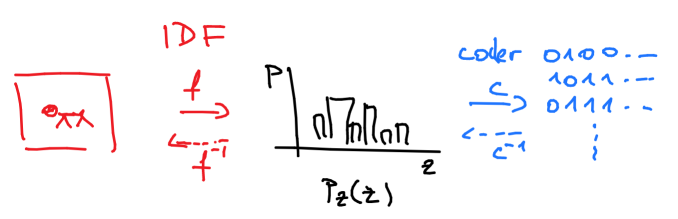
\includegraphics[width=0.7\textwidth]{idf_coding}
\centering
\caption{IDB-based lossless compression: first the data $x \sim p_x$ is passed through the learned IDF $z = f_{id}(x)$ to get to the latent $z \sim p_z$ with known distribution $p_z$, then $z$ is encoded by any off-the-shelf entropy-based encoder (e.g. Huffman, or arithmetic) into the bitstream $c$. For getting $x$ from the bistream $c$, it is first decoded (off-the-shelf) to obtain $z$ and then the inverse IDF maps it to $x = f_{id}^{-1}(z)$.}
\end{figure}

\subsection{Standard flow layers}

Normalizing flows is a stack of density transformations by the change-of-variable formula (e.g. equation \eqref{eqnice:changeOfVar}) using bijective transformations $f_i: \mX_{i} \to \mX_{i+1}$.

They consider:
\begin{compactitem}
\item \textbf{coupling layers}\index{coupling layers} as in realNVPs (section \ref{sec:realNVP}) with splitting $\bx = [\bx_a, \bx_b]$
\begin{gather}
\bz = [\bz_a, \bz_b] = f(\bx) = [\bx_a, \bt(\bx_a) + \bs(\bx_a) \odot \bx_{b}], \quad \bs(\bx_a) \neq 0 \nn
\bx = [\bx_a, \bx_b] = f^{-1}(\bz) = [\bz_{a}, (\bz_{b} - \bt(\bz_a)) \oslash \bs(\bx_a) \nn
\det \frac{\dif \bx}{\dif \bz} = \prod_{i} \bs(\bx_a)_i^{-1} \qquad p_x(\bx) = p_z(f(\bx)) \prod_{i} \bs(\bx_a)_i^{-1}
\end{gather}
\item \textbf{factor-out layers}\index{factor-out layers} also as in realNVPs (section \ref{sec:realNVP}). Here the idea is that not all the dimensions need to be propagated through all the flow layers. Instead part of the dimensions may be \emph{factored-out} at regular intervals and the rest of the flow operates over the remaining lower dimensional data.
For example for two layers we get
\begin{gather}
\bz = [\bz_1, \bz_2]: \quad [\bz_1, \by_1] = f_1(\bx) \qquad \bz_2 = f_2(\by_1) \nn
\bx = f_1^{-1}\big(\bz_1, f_2^{-1}(\bz_2)\big) \nn
p(\bz_1, \by_1) = p(\by_1) p(\bz_1 \vert \by_1) \qquad
p_y(\by_1) = p_{z_2}(f_2(\by_1)) \ \left\lvert \frac{\dif f_2(\by_1)}{\dif \by_1} \right\lvert \nn
p(\bx) = p(\bz_1, \by_1) \left\lvert \frac{\dif f_1(\bx)}{\dif \bx} \right\lvert
= p(\by_1) p(\bz_1 \vert \by_1) \left\lvert \frac{\dif f_1(\bx)}{\dif \bx} \right\lvert
= p_{z_2}(f_2(\by_1)) \ \left\lvert \frac{\dif f_2(\by_1)}{\dif \by_1} \right\lvert
p(\bz_1 \vert \by_1) \left\lvert \frac{\dif f_1(\bx)}{\dif \bx} \right\lvert \nonumber
\end{gather}
This allows for conditional dependence between parts of $\bz$
\begin{equation}
p(\bz) = p(\bz_L) p(\bz_{L-1} \vert \bz_{L})p(\bz_{L-2} \vert \bz_{L}, \bz_{L-1}) \ldots p(\bz_{1} \vert \bz_{2}, \ldots, \bz_{L})
\end{equation}

\end{compactitem}

\subsubsection{Integer discrete flows (IDF)}
For integer-valued observations $\bx \in \mX \in \mzZ^d$ and prior distribution with $p_Z(.)$ with support on $\mzZ^d$ consider a bijection $f : \mzZ^d \to \mzZ^d$ so that
\begin{equation}
p_X(\bx) = p_Z(\bz), \qquad \bz = f(\bx)
\end{equation}
IDF stacks multiple such layers. 

\paragraph{Integer discrete coupling} They design the layers to ensure that the IDF map is closed on $\mzZ^d$ so that they don't have to keep track of the co-domain of $f_{ID}$.
For $\bx = [\bx_a, \bx_b] \in \mzZ^d$
\begin{gather}\label{eqdfc:coupling}
\bz = [\bz_a, \bz_b] = f_{ID}(\bx) = [\bx_a, \bx_{b} + round(\bt(\bx_a))]\nn
\bx = [\bx_a, \bx_b] = f_{ID}^{-1}(\bz) = [\bz_{a}, \bz_{b} - round(\bt(\bx_a))]
\end{gather}
They split $a:b$ as $75\%:25\%$ to apply the rounding to fewer dimensions and have less gradient bias.
The trainable parameters are within the $\bt$ function (a network). To back-propagate through the rounding they use straight through estimator with $\nabla_x(x) = I$.

As the prior distribution $p_Z(.)$ they use the discretized logistic $DLogistic(z | \mu, \sigma)$ which assigns to an integer $z \in \mzZ$ the probability over the interval $[z - 0.5, z + 0.5]$ under the logistic distribution.
\begin{equation*}
DLogistic(z | \mu, \sigma) = \int_{z-0.5}^{z+0.5} Logistic(z' | \mu, \sigma) = F_{logistic}(z+0.5) - F_{logistic}(z-0.5) = \sigma(\frac{z+0.5-\mu}{\sigma}) - \sigma(\frac{z-0.5-\mu}{\sigma})
\end{equation*}

In the factor-out set-up we have for each factoring layer $l$ $p(z_{li} | y_{li}) = DLogistic(z_{li} | \pmb{\mu}(y_{l})_i, \pmb{\sigma}(y_{l})_i)$ where $\pmb{\mu}, \pmb{\sigma}$ are outputs of neural networks (in the implementation it is just one network spitting out $\mu$ and $\log$ scale vectors).

The latent in the last layer $z_L$ has an unconditional learned prior $DLogistic(z_{Li} | \pmb{\mu}_i, \pmb{\sigma}_i)$, where $\pmb{\mu}_i, \pmb{\sigma}_i$ are trainable parameters appearing in the loss through the likelihood evaluation. They also consider a mixture of these where they learn an additional mixing parameter $\pi_i$ (they work with 5 component mixtures.)

\subsection{Architecture}

They split the archi into levels, where each level has a \emph{squeezing operation}\index{squeezing operation}, $D integer flows$ and factor-out layer. Each integer flow consists of permutation (to ensure that all dimensions can interact with all other) followed by a discrete coupling layer. The permutations are initialised once and then kept fixed (not trained).

There is a trade-off between complexity and gradient bias influenced by the number of rounding operations. Instead of increasing the number of IDFs they make more complex the $\bt, \pmb{\mu}$ and $\pmb{\sigma}$ parts of the network.

\subsection{Experiments}

They train IDF over ImageNet32, ImageNet64 and CIFAR10 and then evaluate the likelihood and compression rate over test data ($x \to z = f_{id}(x) \to c = encode(z) \to z'=decode(c) \to x' = f_{id}^{-1}(z')$). I'm guessing the bits per dimension they mention is the $log_2$ likelihood values per pixel $d$ in the input space $\mzZ^d$ evaluated over $x'$ reconstructed from the test data $x$. The compression rate is probably the length of encodings $c$ of the test data compared to some naive encoding $c'$. Perhaps $L(c', x) = \log_2 n_{test}$?

It seems to beat the standard baselines such as JPEG, PNG, FLIF and Bit-Swap in terms of both, the log-likelihood as well as compression rate.
It even performs well if IDF is trained on other data then the the target distribution (e.g. IDF trained on ImageNet32 and used for ImageNet64 and CIFAR10) datasets.

They also have good results for compressing large images by smaller patches and in progressive decompression.

\textbf{See next page for my understanding of the implementation in their github repository.}

\subsection{My pseudo-code for implementation}
\begin{notebox}
\textbf{What I understood from the pyTorch implementation:}

For the \textbf{forward pass} you:
\begin{compactenum}
\item take $\bx$
\item $\bz \gets squeeze(\bx)$ (fixed transform)
\item repeat D times
\begin{compactitem}
\item $\bz \gets permute(\bz)$ (fixed transform)
\item $\bz \gets coupling(\bz)$ ($[\bz_a, \bz_b + \bt(\bz_a)]$ where $\bt()$ are trained neural networks, one for each D, eating on $\bz_a$ $\bz$ and spitting out an output with the same dimensions as $\bz_b$)
\end{compactitem}
\item $[\bz, \by] \gets split(\bz)$ (split $\bz$ for factoring-out parts of the dims, you won't transform $\by$ any more, $\bz$ will be further transformed)
\item $\mu, \sigma \gets h(\bz)$ where $h$ is a nn with outputs $\mu, \sigma$. These are the parameters of the conditional distribution $p(\by \vert \bz)$ (careful, here the notation is swapped as compared to the description in the paper).
\item evaluate $lpy = \log p(\by | \mu(\bz), \sigma(\bz))$ (this will enter the loss)
\item $\bx \gets \bz$ and goto 2 and repeat N-1 times
\item on the Nth repetition skip 4-6
\item evaluate $lpz = \log p(\bz | \mu, \sigma)$ where $\mu, \sigma$ are learned parameters. These are learned by maximizing the objective function $OF$
\item evaluate the loss: $OF = lpz + \sum lpy$ (the $OF$ is equal to $\log p(\bx)$ when you realize that $\bz$ and $\by$'s are different dimensions of a single latent variable living in $\mzZ^d$, the same as $\bx \in \mzZ^d$.)
\end{compactenum}

Train by standard backpropagation. Once trained, you can pass in an input $\bx$ and the $OF$ is its log-likelihood - \emph{you can evaluate the likelihood of your data points}. \\

For \textbf{sampling} you:
\begin{compactenum}
\item sample $\bz ~ p(\bz | \mu, \sigma)$, where $\mu, \sigma$ are the trained (now fixed parameters)
\item repeat D times
\begin{compactitem}
\item $\bz \gets inversecoupling(\bz)$ ($[\bz_a, \bz_b - \bt(\bz_a)]$ where $\bt()$ are the trained neural networks)
\item $\bz \gets inversepermute(\bz)$ (fixed transform)
\end{compactitem}
\item $\bz \gets unsqueeze(\bx)$ (fixed transform)
\item get parameters $\mu(\bz), \sigma(\bz) \gets h(\bz)$ where $h$ is the trained nn
\item sample $\by \sim p(\by | \mu(\bz), \sigma(\bz))$
\item stack $[\bz, \by]$ and go to 2 and repeat N times (perhaps N-1 times?)
\end{compactenum}
Once you have done this N times the length of your stackings $[\bz, \by_1, \ldots, \by_N]$ should be the same as of $\bx$ and you will get a sample of the data $\bx$ by performing the last inverse coupling, inverse permutaions and unsqueezing. \\

\textbf{Following the above pseudo-algo, I should be able to implement this. ;)}
\end{notebox}




\clearpage

\section{Kingma's VAE with inverse autoregressive flows}\label{sec:iaf}

\begin{notebox}
\textbf{Paper: } \fullcite{kingmaImprovedVariationalInference2016}

\hfill Notes taken: 22/2/2020 \index{February 2020}
\end{notebox}

\begin{notebox}
\tldr 
The aim is to increase the flexibility of the approximate posterior (the inference model) $q(\bx \vert \bx)$ in standard VAEs through normalizing flows on $\bz$. \\

Standard Guassian autoregressive models build the random variable $\by = \{y_i\}_{i=1}^D$ by fixing an order in the dimensions and then getting the dimensions one by one as transformation of some easy to sample random variable $\pmb{\epsilon} = \{\epsilon_i\}_{i=1}^D$ (this is not the data here!).
\begin{equation}
\by = \pmb{\mu} + \pmb{\sigma} \pmb{\epsilon}
\end{equation}
\begin{equation}
y_0 = \mu_0 + \sigma_0 \, \epsilon_0, \quad y_i = \mu_i(\by_{1:i-1}) + \sigma_i(\by_{1:i-1}) \, \epsilon_i, \ i=1, \ldots D-1
\end{equation}
with not-autoregressive $\mu_0, \sigma_0$ and $\mu_i, \sigma_i$ being the outputs of some autoregressive network.

The problem with this is that the sampling is slow (you need to sample recursively). Hence this is not very practical in VAEs with high dimensional latent space $\bz$ because there we need to sample the $\bz$ every time we do a forward pass for each of the inputs $\bx$. \\

The \emph{inverse autoregressive flows} (IAF) say you should flip the dependency so that
\begin{equation}
\by = \pmb{\mu} + \pmb{\sigma} \pmb{\epsilon}
\end{equation}
\begin{equation}
y_0 = \mu_0 + \sigma_0 \, \epsilon_0, \quad y_i = \mu_i(\pmb{\epsilon}_{1:i-1}) + \sigma_i(\pmb{\epsilon}_{1:i-1}) \, \epsilon_i, \ i=1, \ldots D-1
\end{equation}
This is much faster to sample (can be parallelized) and the Jacobian is still triangular with simple terms on the diagonal (just $\sigma_i(\pmb{\epsilon}_{1:i-1})$) so that the induced density $p(\by)$ is easy to evaluate.
\end{notebox}

\subsection{Intro}

The aim is to improve VAE's\index{VAE} by increasing the flexibility of the inference model $q(\bz \vert \pmb{\epsilon})$ (so that the approximate posterior $q(\bz \vert \pmb{\epsilon})$ can be closer to the true posterior $p(\bz \vert \pmb{\epsilon})$) through \emph{inverse autoregressive flows} (IAF)\index{inverse autoregressive flows}.

\subsubsection{Normalizing flows}

Build posterior $q(\bz \vert \pmb{\epsilon})$ by starting off an initial random variable $\bz_0$ with known density and distribution which is easy to sample from and apply a chain of invertible transformations $f_t$ such that the last iterate $\bz_T$ has more flexible distribution
\begin{equation}
\bz_0 \sim q(\bz_0 \vert \pmb{\epsilon}), \qquad \bz_t = f_f(\bz_{t-1, \pmb{\epsilon}}), \ t=1, \ldots, T
\end{equation}
\begin{equation}
\log  q(\bz_T \vert \pmb{\epsilon}) = \log q(\bz_0 \vert \pmb{\epsilon}) - \sum_{t=1}^T \log \left\lvert \det \frac{\dif \bz_t}{\bz_{t-1}} \right\rvert
\end{equation} 

\subsection{Inverse autoregressive transformation}

The idea is based on Gaussian autoregressive functions. The variable $\by = \{y_i\}_{i=1}^D$ is modelled as a transformation of an easy to sample random variable $\pmb{\epsilon} = \{\epsilon_i\}_{i=1}^D$ as
\begin{equation}
\by = \pmb{\mu}(\by) + \pmb{\sigma}(\by) \, \pmb{\epsilon} \enspace ,
\end{equation}
where $\pmb{\mu}(\by)$ and $\pmb{\sigma}(\by)$ denote the autoregressive functions so that
\begin{equation}
y_i = \mu_i(\by_{1:i-1}) + \sigma_i(\by_{1:i-1}) \, \epsilon_i, \quad y_0 = \mu_0 + \sigma_0 \, \epsilon_0 \enspace .
\end{equation}


The computational cost of sampling is proportional to the dimension $D$ as we need to iteratively follow from the ancestral dimensions.
However, the determinant of the Jacobian $\frac{\partial \by}{\partial \by}$ is trivial. The Jacobian is lower triangular with zeros on the diagonal because
\begin{equation}\label{eqiaf:autoregressJacob}
\frac{\partial [\mu_i(\by_{1:i-1}), \sigma_i(\by_{1:i-1})]}{\partial y_j} = [0, 0] \quad \text{ for } i \leq j \enspace .
\end{equation}


The inverse transformation
\begin{equation}
\pmb{\epsilon} = \frac{\by - \pmb{\mu}(\by)}{\pmb{\sigma}(\by)}
\qquad 
\epsilon_i = \frac{y_i - \mu_i(\by_{1:i-1})}{\sigma_i(\by_{1:i-1})}
\end{equation}
can be panellized for sampling since the computation of dimensions of $\pmb{\epsilon}$ does not depend on each other.
This transformation has a simple Jacobian determinant as the Jacobian $\partial \pmb{\epsilon} / \partial \by$ is lower triangular with $\partial \epsilon_i / \partial y_j = 0$ for $j > i$ and a simple diagonal $\partial \epsilon_i / \partial y_i = 1 / \sigma_i(\by_{1:i-1})$.
The log determinant is hence simply
\begin{equation}
\log \left\lvert \det \frac{\partial \pmb{\epsilon}}{\partial \by} \right\rvert = - \sum_{i=1}^D \log \sigma_i(\by_{1:i-1})
\end{equation}

\subsection{Inverse autoregressive flows}

They bring the inverse transform into the VAE's as follows:
\begin{compactitem}
\item let the encoder spit out initial $\pmb{\mu}_0, \pmb{\sigma}_0, \bh$
\item initialize chain by $\bz_0 = \pmb{\mu}_0 + \pmb{\sigma}_0 \, \pmb{\epsilon}$, with $\pmb{\epsilon} \sim N(\mathbf{0}, \mathbf{I})$
\item construct flow as the chain of transformations $\bz_t = \pmb{\mu}_t(\bz_{t-1}, \bh) + \pmb{\sigma}_t(\bz_{t-1}, \bh) \, \bz_{t-1}$ with autoregressive $\pmb{\mu}_t, \pmb{\sigma}_t$ outputs of an autoregressive neural network.  
\end{compactitem}
Jacobians of $\partial [\pmb{\mu}_t(\bz_{t-1}, \bh), \pmb{\sigma}_t(\bz_{t-1}, \bh)] / \partial \bz_{t-1}$ are triangular with zeros on the diagonal so that the Jacobian of each of the transformation is triangular with $\partial \bz_t / \partial \bz_{t-1} = \pmb{\sigma}_t(\bz_{t-1}, \bh)$ on the diagonal.

For gaussian $\pmb{\epsilon}$ the density of the final iterate is
\begin{equation}
p(\bz_T \vert \pmb{\epsilon}) = - \sum_i^D \left( 
0.5 \epsilon_i^2 + 0.5 \log(2\pi) + \sum_{t=0}^T \log \sigma_{t,i}(\bz_{t-1})
\right)
\end{equation}
\note{Is this a Gaussian distribution with diagonal covariance? It should not be but the density looks like it is.}

\subsection{Implementation tricks}
They use MADE \parencite{germainMADEMaskedAutoencoder2015} and PixelRNN \parencite{oordPixelRecurrentNeural2016} as the autoregressive networks for the flow. They also use a numerically more stable version of the flow transformation
\begin{equation}
[\bm_t, \bs_t] \gets autoregressNN(\bz_t, \bh) \quad \pmb{\sigma}_t = sigmoid(\bs_t) \quad \bz_t = \pmb{\sigma}_t \odot \bz_{t-1} + (1 - \pmb{\sigma}_t) \odot \bm_t \enspace .
\end{equation} 
\note{I'm not sure of the role of $\bh$ which is being used as an input into all the flow layers.}

\subsection{Experiments}
They compare to baselines (results taken from other papers) over MNIST and CIFAR and show that likelihood (by importance sampling) is competitive and the generations can be much faster than that of standard autoregressive models such as PixelCNN. 


\clearpage 

\section{Ardizzone: Inverse problems through invertible networks}\label{sec:inverseProblem}

\begin{notebox}
\fullcite{ardizzoneAnalyzingInverseProblems2019}

\hfill Notes taken: 24/2/2020 \index{February 2020}
\end{notebox}

\begin{notebox}
\tldr You know from some physical model the forward function $\by = s(\bx)$ which allows you to simulate data. However, this does not mean that from the observations of $\by$ you can recover $\bx$ (the inverse problem). They propose to learn the inverse function $f^{-1}$ via invertible network ensuring that the learned forward approximates the simulator $f \approx s$. \\

The simulator may not be invertible (mathematically). Instead of learning a deterministic transformation $\bx = f^{-1}(\by)$ they therefore learn a probabilistic mapping $q(\bx| \by)$ where the conditional distribution is implied by a deterministic function $g(\by, \bz; \theta)$ with a random variable $\bz \sim \mathcal{N}(0, I)$. \\

They pose it into the invertible architecture so that they get $g^{-1}(\bx) = f(\bx; \theta) = [f_y(\bx; \theta), f_z(\bz; \theta)]$ with single parametrization. They use the standard change of variable formulas to recover the density $q(\bx| \by)$ and optimize the forward pass as well as the backward pass with a different losses (checking the prediction of $\by$ compared to the ground truth and checking the normality of $\bz$ and its independence from $\by$ respectively.)
\end{notebox}

If you know the \emph{forward function}\index{forward function} (e.g. simulator) $\by = s(\bx)$ which generates some observables $\by$ from some hidden parameters, it does not mean we also know the inverse function $s^{-1}$ to get the hidden parameters $\bx$ from the observed $\by$.

Nice example: $\bx$ are the parameters of a robotic arm (vertical location along a rail and 3 angles in 3 joints), $\by$ is the location (in 2D) where the arm reached. I can easily model the arm and get the location $\by = s(\bx)$. However, it is not obvious to get the setting of the parameters $\bx$ for a known location $\by$. Or rather, there are many possible and what they want to infer is the posterior distribution $p(\bx | \by)$ over these. 

I find this a bit ill posed because in the set-up above, there is no reason why there should be some other than uniform distribution over all possible configurations. Hm, but in the marginals perhaps some configurations can be more probable because they can combine with multiple configurations of the other parameters? And there is certainly plenty of dependencies.

They formulate it as a flow network where they 
\begin{compactitem}
\item assume latent variable model with $\bz \sim p(\bz) = \mathcal{N}(0, I_K)$ and $\bx = g(\by, \bz; \theta)$ where we learn the deterministic function $g$ as a neural network
\item by the standard change of variable we get for the conditional density
\begin{equation}\label{eqinverse:conditional}
q(\bx | \by) = p(\bz) \, \big\lvert \det J_x \big\rvert^{-1}, \quad 
J_x = \frac{\partial g(\by, \bz; \theta)}{\partial [\by, \bz]} \Bigg\rvert_{\by, f_z(\bx)}
\end{equation}
\item approximate the known forward function by learned $f_y(\bx; \theta) \approx s(\bx)$ and learn it jointly with the inverse process
\begin{equation}
[\by, \bz] = [f_y(\bx; \theta), f_z(\bx; \theta)] = f(\bx; \theta) = g^{-1}(\bx)
\end{equation}
tying together the parameters $\theta$ by the architecture of the invertible network. 
\end{compactitem}

There will be some problems with the dimensionality of the $\bx$ and $[\by, \bz]$ which normally should match but they propose to solve it simply by padding (and some more hacks, I think).

They then use a variant of the \emph{coupling layers}\index{coupling layers}, actually also interesting because it does not pass part of the inputs unchanged. Instead it changes everything but needs to do the updates and the inverses sequentially
\begin{equation}
\bv_1 = \bu_1 \odot exp(s_2(\bu_2)) + t_2(\bu_2), \qquad
\bv_2 = \bu_2 \odot exp(s_1(\bv_1)) + t_1(\bv_1)
\end{equation}
with the inverse
\begin{equation}
\bu_2 = (\bv_2 - t_1(\bv_1)) \odot exp(-s_1(\bv_1)), \qquad
\bu_1 = (\bv_1 - t_2(\bu_2)) \odot exp(-s_2(\bu_2))
\end{equation}

The loss is not a simple maximum likelihood.
Instead they do bi-derctional training where they accumulate the gradients from the forward and backward iterations and corresponding losses and only update after.
\begin{compactitem}
\item For the forward iteration the loss penalizes deviations of the network predictions from the simulations $L_y(f_y(\bx), s(\bx))$. This can be something like squared error or cross entropy.
\item For the backward iteration the loss penalizes the mismatch between the joint latent distribution and the product of their marginals $L_z(q(\by, \bz), p(\by), p(\bz)) = MMD(q(\by, \bz), p(\by), p(\bz))$, where
$p(\bz)$ is the normal prior, $p(\by = s(\bx)) = p(\bx) \, \big\lvert \det J_s \big\rvert^{-1}$ with $J_s = \partial s(\bx) / \partial \bx$ and $q(\by = f_y(\bx), \bz= f_z(\bz)) = p(\bx) \big\lvert \det J_f \big\rvert^{-1}$ with $J_f = \partial f(\bx) / \partial \bx$.
Here $p(\bx)$ is some fixed prior distribution.
This ensures that $\by, \bz$ are independent and that the generated $\bz$ follows the normal distribution.
As the distance measure $MMD$\index{MMD} they use the \emph{Maximum Mean Discrepency}\index{Maximum Mean Discrepency} which can be evaluated efficiently over data samples
\item To speed up convergence they add a third loss $L_x(p(\bx), q(\bx)) = MMD(p(\bx), q(\bx))$, where $q(\bx) = p(\by = f_y(\bx))p(\bz = f_z(\bx)) \big\lvert \det J_x \big\rvert^{-1}$ with $J_x$ as in equation \eqref{eqinverse:conditional}.
\end{compactitem}

The experiments compare the MAP estimates of the $\bx$ as well as the distributions through \emph{calibration error}\index{calibration error} (something to do with the proportion of true data within a confidence interval) and they plot the marginal posterior densities to show how they deviate from the priors $p(\bx)$ (the kernel density estimate over the data?)





\clearpage 

\section{Kumar et al.: VideoFlow}\label{sec:videoFlow}

\begin{notebox}
\fullcite{kumarVideoFlowConditionalFlowBased2020}

\hfill Notes taken: 24/6/2020 \index{June 2020}
\end{notebox}

\begin{notebox}
\tldr They use flow model to predict future video frames. They argue by the usual advantages of flows as compared to VAEs, GANs and autoregressive (explicit likelihood, easier training, faster generations). The flows operate over individual frames (usual realNVP and Glow architecture and tricks) and the temporal dependence is only factored into the latent distribution $p_{\theta}(\bz)$ via temporal autoregressive probability model. 
\end{notebox}

The aim is stochastic prediction of video sequences - synthesizing RGB video frames conditioned on a few previous frames. Unlike previous work for video generations the flow-based model can generate diverse stochastic futures (as opposed to deterministic models) relatively cheaply (as compared to autoregressive models) and at the same time provide exact likelihood estimates (as opposed to VAEs or GANs).

Points out standard disadvantages of other generative models (VAEs \& GANs lack of likelihood estimtes, GANs difficult to train, autoregressive slow to sample/generate). Moreover previously proposed \emph{deterministic} models for video generation can only generate single future which either disregards other possibilities or mixes all of them into a blurry single future.

They use flow model for each frame with architectural tricks similar to Glow (section \ref{sec:Glow}) with multi-scale architecture as in realNVP (section \ref{sec:realNVP}). To account for the time-dependency between frames they make the prior over the latent $\bz$ autoregressive conditioning on the previous frames
\begin{gather}
p_\theta(\bz) = \prod_{t=1}^T p_\theta(\bz_t | \bz_<t) \\
p_\theta(\bz_t | \bz_{<t}) = \prod_{l=1}^L p_\theta(\bz_t^{(l)} | \bz_{<t}^{(l)}, \bz_t^{(>l)}) = \mathcal{N}(\bz_t^{(l)} ; \mu, \sigma) \\
(\mu, \log \sigma) = \text{neural net}_\theta(\bz_{<t}^{(l)}, \bz_t^{(>l)})
\end{gather}
where $<t$ indicates previous time frame, $>l$ indicates higher levels at the multi-scale architecture and the neural net is a 3D residual network \note{see Fig10 in paper for sketch of architecture}.
This means that the temporal dependency between the video frames is factored into the model by the autoregressive structure in the latent prior while the flow model acts on individual frames. They claim making the flow temporal via 3D convolutions was too expensive to train.

The experiments show comparable or slightly better results compared to stochastic VAE or GAN based models in video prediction in terms of Frechet Video Distance, better in likelihood. However, they are quite honest in the evaluation showing also less good results such as accuracy of best prediction and failures for more complex dataset such as human motion videos (in the appendix).

They typically condition on only 1-3 previous frames and then generate up to 100 future frames. I wonder why they condition on so little data, I'm guessing computational complexity in combination with these datasets being such that only few frames give enough info for the future. Perhaps true for most datasets, needs some thinking.



\clearpage

\section{Short dirty notes for more papers}


\subsection{Rippel, Adams: High dimensional density estimation}

\begin{notebox}
\fullcite{rippelHighDimensionalProbabilityEstimation2013}

\hfill Notes taken: 22/2/2020 \index{February 2020}
\end{notebox}

Good review of various density estimation methods organised in tow groups:
\begin{compactitem}
\item graphical models, e.g. Boltzmann machine, directed belief networks, etc.
\item manifold learning, e.g. Gaussian latent variable model, kernel PCA, auto-encoder neural network
\end{compactitem}
Inference is often costly and not scalable to high dimensions.
They propose the \emph{deep density model} (DDM)\index{deep density model} using deep learning for bijective transformations of the observed space.

The structure they propose is quite different from modern flow architectures.
They suggested to have an invertible \emph{decoder}\index{decoder} $f_\theta : \mZ \subseteq \mR^D \to \mX \subseteq \mR^D$ such that the transformation of the observed data $f_\theta^{-1} : \mX \to \mZ$ has a simple factorised distribution 
\begin{equation}
p_Z(\bz) = \prod_i^D p(z_i) \enspace .
\end{equation}
The decoder $f$ shall be a stacking of standard sigmoidal layers $\sigma(\bW \bx + \bb)$.

They also have non-bijective \emph{encoder}\index{encoder} $g_\phi : \mX \to \mZ$.

Their objective is composed of three terms:
\begin{compactitem}
\item divergence term making sure that after the encoding transform $g_\phi$ the empirical distribution of the latent representation matches the target distribution of choice. They work with Beta distributions and do this by calculating analytically the KL divergence between the base Beta and the a Beta fit to the empirical $\bz$'s. \note{this seems complicated}
\item invertibility measure which makes sure that the learned $\bW$'s are invertible. This is based on the condition number but as they say, in high dimensions virtually all matrices are orthogonal.
\item Reconstruction loss checking that the encoder-decoder chain reconstructs well. This is based on entropy which I don't really understand why.
\end{compactitem}

They have some interesting ideas for experiments:
\begin{compactitem}
\item to test their density estimation they check the density assigned to train data and test data which should both be high and distorted data which should have low density
\item they train on MNIST digit 9 and check the density for 6 (should be low) and rotated 6 (should be high)
\end{compactitem}

They mention the possiblity to extend to supervised learning with calibrated classificaiton predictions.


\subsection{Germain et al, Masked Autoencoder for Distribution Estimation (MADE)}\index{MADE}

\begin{notebox}
\fullcite{germainMADEMaskedAutoencoder2015}

\hfill Notes taken: 22/2/2020 \index{February 2020}
\end{notebox}

Standard autoencoders over binary data optimizing cross-entropy per dimension are equivalent to maximizing the factorised log likelihood. However, the true distribution is unlikely to be factorised. In contrast, any distribution can be decomposed into the product of \emph{autoregressive} conditionals where the distribution for each dimension is conditioned on the previous dimensions.

They propose to multiply (element-wise) the weight matrices in the encoder and decoder by binary masks that will block the paths so that the outputs only depend on previous dimensions of the inputs. The idea is fairly simple and the trick is only how to construct these automatically so that it actually really blocks the path as needed - they give simple heuristic that can be initialised randomly.

They further make this more complicated by randomly permuting the order of the dimensions during the training when the order has no ture meaning.


\subsection{Oord et al., PixelRNN}\index{PixelRNN}

\begin{notebox}
\fullcite{oordPixelRecurrentNeural2016}

\hfill Notes taken: 22/2/2020 \index{February 2020}
\end{notebox}

Model the distribution of an image by expressing the joint distribution as a product of conditional distributions where we condition the distribution of each pixel on the prevoius pixels (to the left and top).

To model the recurences they use RNN (with LSTM layers) and masked CNN where the filters are masked so that they don't peak to the future pixels.

The paper discusses plenty of architectures for the RNN or CNN models achieving this. But the point is that the images have to be generated sequentially by passing the outputs again and again through the networks to produce more and more pixels.

\subsection{Oord et al., Conditinal generations with PixelCNNs}

\begin{notebox}
\fullcite{oordConditionalImageGeneration2016}

\hfill Notes taken: 22/2/2020 \index{February 2020}
\end{notebox}

Extends the previous PixelCNN\index{PixelCNN} by conditioning all the autoregressive distributions on a common vector $\bh$ giving some high-level description of the image (e.g. class). This can be either global, so used for conditioning all pixels or local and then would be applied only to some pixels through masking.

\subsection{Kingma and Dhariwal: Glow}\label{sec:Glow}\index{Glow}

\begin{notebox}
\fullcite{kingmaGlowGenerativeFlow2018}

\hfill Notes taken: 23/2/2020 \index{February 2020}
\end{notebox}

Good motivation of generative modelling and major pros and cons of flows as compared to autoregressive, VAEs and GANs in the intro.

Very clear intro to flows (hinting to the fact that continuous variables are always discretized by digitalization process so they add uniform noise to the observation to make them continuous again).

Takes realNVP architecture (section \ref{sec:realNVP}) and replaces 
\begin{compactitem}
\item batch norm with \emph{actnorm} - for large images the minibatch has size 1 and therefore batchnorm would be very unstable. Actnorm normalizes initial activations per channel by the mean and std calculated over initial minibatch and then treats these as learnable parameters
\item dimension permutation with invertible 1x1 convolution - this is easy to invert and get Jacobian determinant
\item affine coupling layer with additive layers - in the factor-out architecture they split the features along channels
\end{compactitem}

\textbf{Good experimental results.} They claim the 1x1 convolution does better than random or reverse permutations reaching higher log likelihood values. Generations from CelebA look good.
They also show interpolations in the latent representations and these look very good suggesting the latent space is very smooth. 
They also have a nice trick for semantic manipulation: they simply calculate average latent vectors for images with and without some discrete feature (e.g. smile) and then move along the difference of these two. Looks good.

They speak about somehow reducing the temperature of the model but I'm not sure what temperature they speak about. This seems like post-hoc reduction in the variance of the latent space for neater 4sampling.


\subsection{Ho et al: Flow++}

\begin{notebox}
\fullcite{hoFlowImprovingFlowBased2019}

\hfill Notes taken: 23/2/2020 \index{February 2020}
\end{notebox}

Builds on Glow (secttion \ref{sec:Glow}) and claims that transforming the digitized data to continuous by adding uniform noise (\emph{dequantization}\index{dequantization})
\begin{equation}
\tilde{\bx} = \bx + \bu, \qquad \bu \sim \mathcal{U}(0, 1)^D
\end{equation}
and maximizing the likelihood $p(\tilde{\bx})$ is not great.
It does prevent the model from collapsing to the discrete data, however, it asks the model to assign uniform density to to unit hypercubes around the data $\bx + [0, 1)^D$ which is not natural for a smooth function approximator.

They therefore propose to learn the most reasonable distribution of the additive $\bu$ through approximation $q(\bu | \bx)$ which itself is modelled as a flow $\bu = q_x(\pmb{\epsilon})$, $\pmb{\epsilon} \sim \mathcal{N}(\mathbf{0}, \mathbf{I})$.
Doing this they don't optimize the likelihood but a variational bound but they claim that even the uniform deqauntization boils down to optimizing a variational bound where we approximate the true $p(\bu| \bx)$ by the uniform distribution.

They add some more tweaks to the architecture. They design more complex affine layers with extra invertible nonlinearity babsed on Logistic CDF of the data which requires learning plenty more parameters. They bring attention and gating to the networks acting in the coupling layers. They claim these help but are less important than learning of the $\bu$ distribution.


\subsection{Magdon-Ismail, Atiya: Density Estimation Using Multilayer Networks}

\begin{notebox}
\fullcite{magdon-ismailDensityEstimationRandom2002}

\hfill Notes taken: 23/2/2020 \index{February 2020}
\end{notebox}

Rather old paper. They propose to learn the data distribution via NN as non-parametric class. They rely on the CDF rather than the pdf as pdf is just a derivative of the CDF which should be able to obtain from the neural net.

In the univariate case $x \in \mR$ the r.v. $y=CDF(x)$ is uniform on (0, 1). They propose to learn the nn as the CDF, that is the outputs of the network should be distributed uniformly.
They pose it as a supervised learning problem and to each $x$ they associate an $y \sim Uni(0, 1)$ and optimize the network. They generate new $y$s after every forward-backward pass to allow it to learn a truly uniform distribution not just fit the outputs.

In the multivariate case $\bx \in \mR^d$ the variable $\by = CDF(\bx)$ is not necessarily uniform. \\
(\note{I had though it is still marginally uniform but not independent}).
They construct targets for the learning as the fraction of the training data smaller than each of the training points. 
The density is simply the derivatve of the learned CDF.


\subsection{Uria, Murray, Larochell: RNADE}

\begin{notebox}
\fullcite{uriaRNADERealvaluedNeural2014}

\hfill Notes taken: 23/2/2020 \index{February 2020}
\end{notebox}

Good review of traditional approaches to density estimation in the intro.

Extends previous Neural Autoregressive Distribution Estimator\index{neural autoregressive distribution estimator} (NADE)\index{NADE} which modelled discrete distribution to the continuous case.

The model is autoregressive relying on the generally valid decomposition of probability density by the product rule (chain rule)\index{product rule}\index{chain rule}
\begin{equation}
p(\bx) = p(x_1) \prod_{d=2}^D p(x_d \vert \bx_{<d})
\end{equation}

In NADE each conditional is given by a feed-forward neural net with one hidden layer $\bh_d \in \mR^H$
\begin{equation}
p(x_d \vert \bx_{<d}) = sigm(\bv_d^T \bh_d + b_d), \qquad \bh_d = sigm(\bW_{<d} \bx_{<d} + \bc) \enspace .
\end{equation}
The parameters are tied across the dimensions with $\bW_{<d}$ being the first $d-1$ columns of a shared weight matrix $\bW$.

For the Real-valued neural autoregressive distribution estimator\index{real-valued neural autoregressive distribution estimator} (RNADE)\index{RNADE} the conditionals are modelled as mixture of Gaussians  so that the outputs of the network are the mixing fractions (softmax), component means and component standard deviations ($\log \sigma$).
Otherwise the architecture pretty much follows NADE including the parameter tying.
The architecture is a rather shallow network, probably due to the date of drafting and comp resources available at the time.

In addition to mixture of Gaussian they also tried mixture of Laplacians, claiming it may be more appropriate for some types of data.
They only experimented with relatively low diemansional data and compared to simple baselines such as mixture of Gaussians optimised by EM and it performed reasonably well.

\subsection{Papamakarios, Pavlakou, Murray: MAF}

\begin{notebox}
\fullcite{papamakariosMaskedAutoregressiveFlow2018}

\hfill Notes taken: 23/2/2020 \index{February 2020}
\end{notebox}

View autoregressive model as a normalizing flow and use MADE\index{MADE} to avoid the sequential looping. Can stack multiple autoregressive flows on top of each permuting the order of the dimensions which breaks the arbitrary ordering creating troubles in autoregressive models.

After stating the main idea it shows how the autoregressive models can be interpreted as flows and how this links to inverse autoregressive flows of Kingma (section \ref{sec:iaf}).

Experiments are not amazing so seem more honest. Also does conditional density estimation and generation by conditioning all the densities in the autoregression on an side variable $y$ by $p(\bx | \by) = p(x_1 | \by) \prod_{d=2}^D p(x_d \vert \bx_{<d}, \by)$


\subsection{Wang, Wang: Neural Gaussian Copula for Variational Autoencoders}

\begin{notebox}
\fullcite{wangNeuralGaussianCopula2019}

\hfill Notes taken: 23/2/2020 \index{February 2020}
\end{notebox}

They argue that one of the problems in VAEs is the mean field assumption for the approximate posterior $q(\bz | \bx)$. They propose to use copulas\index{copula} to capture the dependencies. Though the idea of using copulas in general may be interesting, in their case I don't see the beauty because it essentially boils down to learn $q(\bz | \bx) = N(\mu(\bx), \Sigma(\bx))$ with full covariance matrix where $\Sigma(\bx) = L(\bx)^T L(\bx)$ are outputs of the NN.


\subsection{Weise et al.: Copula and Marginal flows}

\begin{notebox}
\fullcite{wieseCopulaMarginalFlows2019}

\hfill Notes taken: 23/2/2020 \index{February 2020}
\end{notebox}

I don't think I understand. 
They first that you distribution estimate should coincide with the true distribution in cumulative distribution function and that if you have some tail beliefs you should be able to factor them in.

Then they show that current flows do not necessarily learn the tail probabilities satisfactorily (I don't understand the proofs).

Then they suggest to model the density as the product of copula\index{copula} and marginal densities
\begin{equation}\label{eqmix:copulMarginals}
p(x_1, x_2) = p(x_2 | x_1) p(x_1) = c(F_1(x_1), F_2(x_2)) p(x_1) p(x_2) \enspace ,
\end{equation}
where $c$ is the copula density and $F_i$ are the marginal cumulative distribution functions.

They then propose flows for the marginals and the copula. Somehow it seems to me that they assume you know the copula over the uniform vector $u_i = F_i(x_i)$ a priori and you just need to flow it through and combine with the data distribution.

They only develop and experiment with bivariate case but claim this can be extended to higher dimansions via vine copula.


\subsection{Tagasovska et al.: Copulas as High-Dimensional Generative Models}

\begin{notebox}
\fullcite{tagasovskaCopulasHighDimensionalGenerative2019}

\hfill Notes taken: 24/2/2020 \index{February 2020}
\end{notebox}

Train normal neural autoencoder with lower-dimensional latent space and learn a copula\index{copula} distribution over the latent space (post-hoc) to be able to generate new data by decoding the $z$ samples.

They use the same density representation as above in equation \eqref{eqmix:copulMarginals} (product of copula density and the marginals) generalizing to $d>2$ variables.
To estimate the marginals they use Gaussian kernel density estimation.
They use parametric and non-parametric (claim this is better since more flexible) vine copulas based on pair-copula constructions (pair-wise dependencies conditioned on other variables) to estimate the copula density. The standard estimation procedure is sequential constructing \emph{conditioned pseudo-observations} to be able to evaluate the conditional copulas. This somehow reminds me of autoregressive  models but I'm not quite sure about the link.
They use the R implemented rvinecopulib to do the estimation.


\subsection{Dinh et al.: RAD}\index{RAD - Real And Discrete flow}

\begin{notebox}
\fullcite{dinhRADApproachDeep2019}

\hfill Notes taken: 24/2/2020 \index{February 2020}
\end{notebox}

Flow model where they intorduce an extra latent variale $k$ which shall cater for multiple modes (clusters) in the data. The flow transformation $f$ thus has to be no-longer invertible but only piecewise invertible over partitions of data associated to the invidual clusters. They consider the partitions to be disjoint (means hard-clustering / strict separation which seem quite strong and restrictive assumption). 

Otherwise just extending RealNVPs (section \ref{sec:realNVP}) with the extra $f_K$ clustering function. They not this is difficult to optimise due to discontinuities but they say they solve it by gating layers. Not sure how.

On experiments seems to perform better than standard RealNVP


\subsection{Tabak and Turner: Family of Nonparametric Density Estimation Algos}

\begin{notebox}
\fullcite{tabakFamilyNonparametricDensity2013}

\hfill Notes taken: 24/2/2020 \index{February 2020}
\end{notebox}

One of the original normalizing flow papers.
Suggests to maximize the likelihood via the parametrized flow map $x = f_\beta(z)$ from a standard Gaussian latent $\bz$.
They also propose to stak the transformations to combine simple transforamtions into something more complex. However, they don't go around it by NN but rather something that looks like kernel density estimation. 

\subsection{Ardizzone: Guided image generation, conditional INN}

\begin{notebox}
\fullcite{ardizzoneGuidedImageGeneration2019}

\hfill Notes taken: 24/2/2020 \index{February 2020}
\end{notebox}

Builds upon their paper on inverse problems (section \ref{sec:inverseProblem}).
It proposes conditional generations where the condition enters directly as inputs to the $t()$ and $s()$ networks in the coupling layers (this is ok, since these are not iverted). This is easy for something like MNIST and the class one hot vectors. For something more complicated, the condition (e.g. image) may need to be pre-processed by a conditioning network, either some pre-trained network allowing to extract reasonable features or trained together directly with the cINN.
For MNIST they train with $c$ the one-hot vectors for the digit classes and can then conditionally generate from each digits tweaking the style by changing $\bz$. They can do the reverse in fixing the style in $\bz$ and change $c$ to generate different digits or even style transfer by passing $\bx$, getting the corresponding $\bz$ and changing $\bc$.

They also tweak the style of the single digits by moving in the $\bz$ space along PCA latent vectors (learned post-hoc over $\bz$s of training data).

They have another experiment on coloring images where the conditioning info is the grayscale image and the colorization comes from learned distribution. I don't quite understand how this works (what is \emph{Lab color space}?) but the results seem rather impressive to me. Not so much to ICLR reviewers, it seems ;)



\clearpage 
\printbibliography



% print index
\phantomsection
\cleardoublepage
\addcontentsline{toc}{section}{\indexname}
\printindex

\end{document}
